\subsection*{3.3\quad 机器学习基础}
\subsubsection*{3.3.1\quad 关键对象与术语}
\noindent \textbf{一\quad 任务 数据与样本\quad 基本对象与形式化表示}

\noindent 机器学习研究的直接对象是学习问题的形式化表达,而不是孤立的算法技巧。一个学习系统要成立,首先必须明确三件事。系统要完成的任务是什么,系统将从何种经验中改进,以及用何种性能度量来判定改进是否发生。任务给出输出的语义与形式,经验规定可用于学习的信息来源,性能度量则决定训练与比较模型时好坏的标尺。三者共同构成学习问题的边界条件。边界不清,训练过程即便收敛,也可能是在优化与真实目标不一致的替代目标。

\noindent 在形式化层面,最常用的表达是区分输入与输出。通常用 $X$ 表示输入数据,常见形式是特征矩阵或设计矩阵,用 $y$ 表示输出数据,也就是目标、标签或响应。$X$ 表示预测时可获得的描述信息,$y$ 表示训练阶段用作监督信号而在预测时不可直接使用的目标信息。以房价预测为例,$X$ 可以包含面积、户型、地段、楼龄、周边配套等属性,$y$ 是成交价格。训练阶段模型观察 $(X, y)$ 来学习映射规律。部署阶段模型仅接收新的 $X$,输出预测值 $\hat{y}$。这一区分看似只是符号约定,实质上规定了信息可得性的硬约束。任何预测时无法获得的信息,都不应被纳入 $X$。如果把未来信息或与目标几乎同义的字段混入特征,离线指标往往会异常乐观,而上线表现会迅速变差。

\noindent \begin{figure}[htbp]
\centering
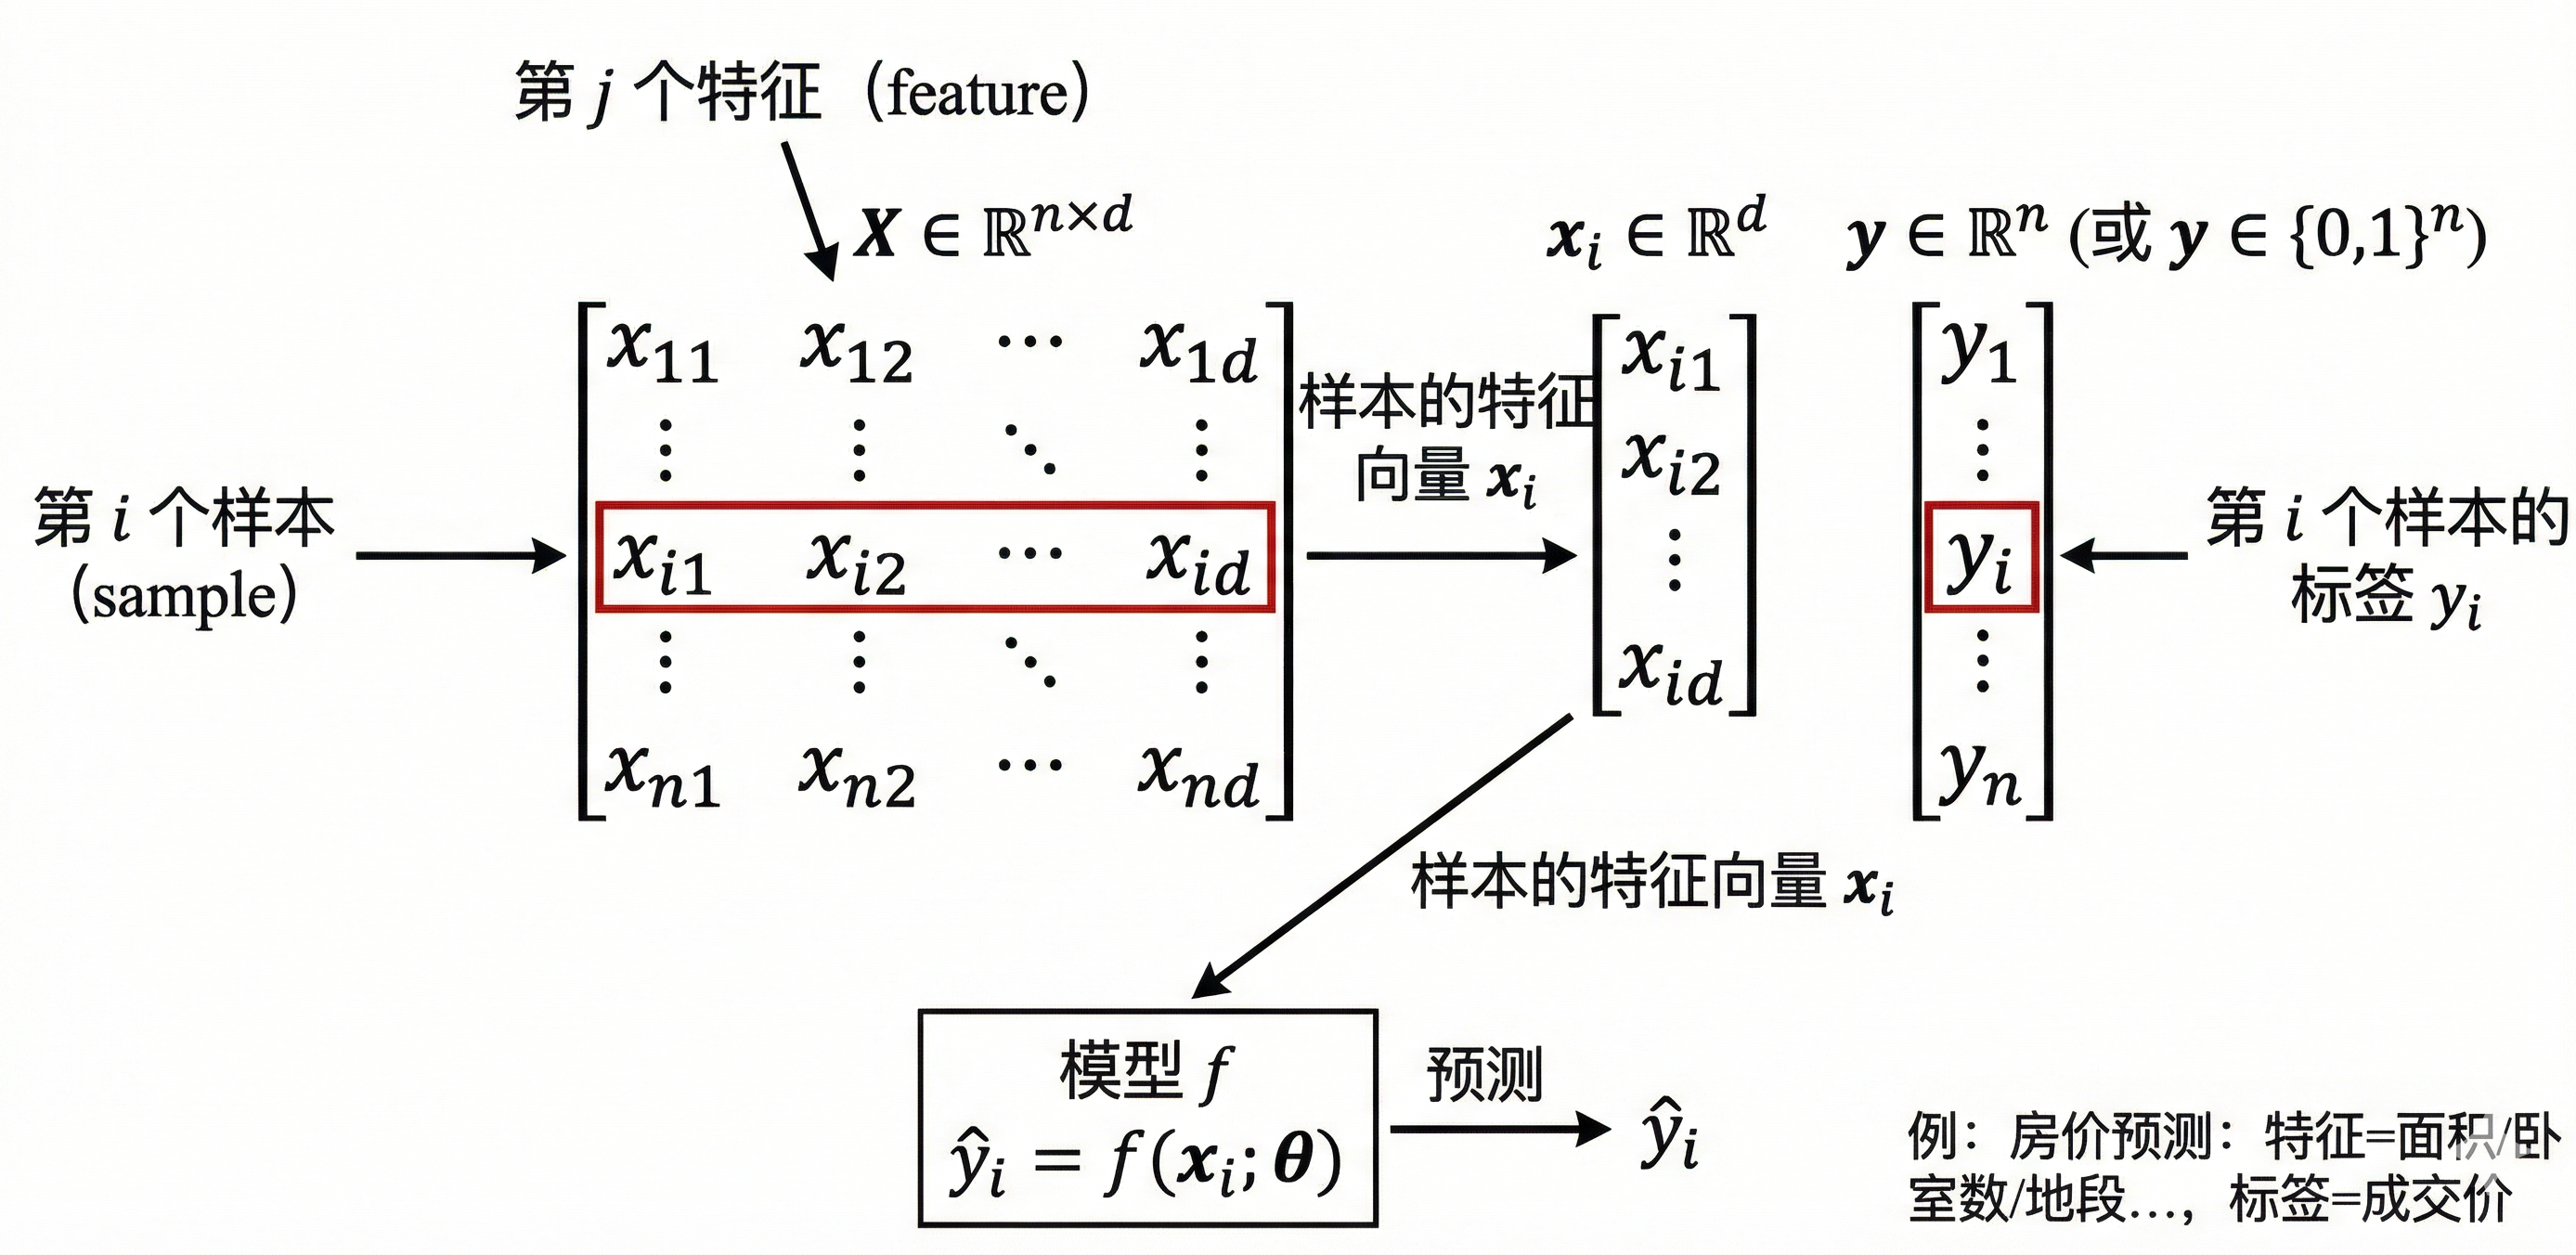
\includegraphics[width=0.75\textwidth]{figures/fig-3-3-1-input-output.png}
\caption{输入$X$与输出$y$的关系示意图}
\label{fig:3-3-1-input-output}
\end{figure}

\noindent 在 $X$ 与 $y$ 的表示下,数据集由大量样本组成。样本是学习与评估的基本单位,通常对应 $X$ 的一行,也就是一个输入实例的特征向量。特征对应 $X$ 的一列,表示对所有样本以同一规则测量或抽取的属性。仍以房价为例,每套房子是一条样本,面积、卧室数、是否学区房是不同特征。将数据组织为矩阵并非为了形式美观,而是为了把异质对象统一成可计算的表示,从而使学习一个从 $X$ 到 $y$ 的映射成为明确的数学问题。

\noindent 监督学习中的标签应被视为一种观测结果,而不是天然真值。很多任务的标签来自人工标注、业务规则或延迟反馈,因此不可避免地包含噪声、口径不一致以及随时间变化的漂移。以垃圾信息识别为例,$X$ 可由邮件正文、标题、发件域名、历史交互等构成,$y$ 为垃圾或非垃圾。对于边界邮件,不同标注者或不同时期的策略可能给出不同结论。这类不一致会直接体现在模型可达到的上限与误差形态之中。因此,标签定义的清晰性、稳定性与可复现性,是模型性能与实验可信度的前置条件,而不是训练之后才考虑的附属问题。

\noindent 训练与评估的分离是学习问题成立的基本要求。用同一批数据既训练又评估,会把对已见样本的拟合误当作对未见样本的能力,从而得到系统性偏高的结论。实践中通常将数据划分为训练集、验证集与测试集。训练集用于拟合模型参数,验证集用于模型选择与超参数调节,测试集用于对最终模型给出尽可能无偏的泛化估计。需要强调的是,分离不仅发生在模型训练层面,也必须贯穿所有会从数据中估计统计量的步骤。以标准化为例,如果先用全量数据计算均值与方差再切分数据,测试集的信息已经通过统计量渗入训练过程。类似风险同样存在于缺失值填充、特征选择、降维、目标编码等预处理之中。可靠的流程是先切分,再在训练数据上拟合预处理参数,并把同样的变换仅应用到验证集与测试集上。

\noindent 此外,样本之间并不总是相互独立。现实数据常存在同源相关性,例如同一用户的多次行为、同一设备的连续监测窗口、同一患者的多次影像检查等。如果这些高度相关的样本同时出现在训练集与测试集,模型可能通过记住实体特征取得高分,而在真正的新实体上表现明显下降。以医疗影像为例,如果同一患者的多张 X 光片分散到训练与测试中,模型可能利用与病灶无关但与患者个体相关的低层纹理或成像条件获得虚高的测试成绩。因而,数据划分策略应与泛化目标一致。当目标是对新用户、新设备或新时间段泛化时,划分就应避免相关样本跨集合混入,从评估机制上保证测试集确实代表未见条件。

\noindent 通过上述概念体系,学习问题获得了统一而严格的表述。用 $X$ 描述可用输入,用 $y$ 定义监督目标,以样本与特征的矩阵结构组织数据,并通过训练、验证、测试的隔离流程约束评估可信度,同时在必要时显式处理样本相关结构对泛化判断的影响。后续关于模型、损失函数与优化方法的讨论,均以这些基本对象与表示为基础展开。

\noindent \textbf{二\quad 模型、假设空间、参数与超参数}

\noindent 为使概念精确且便于落地,本节使用同一例子贯穿,用线性模型预测房价。设输入为特征向量 $x \in \mathbb{R}^d$,输出为真实价格 $y \in \mathbb{R}$。训练数据集记为
$\mathcal{D}=\{(x_i,y_i)\}_{i=1}^n$。

\noindent \begin{figure}[htbp]
\centering
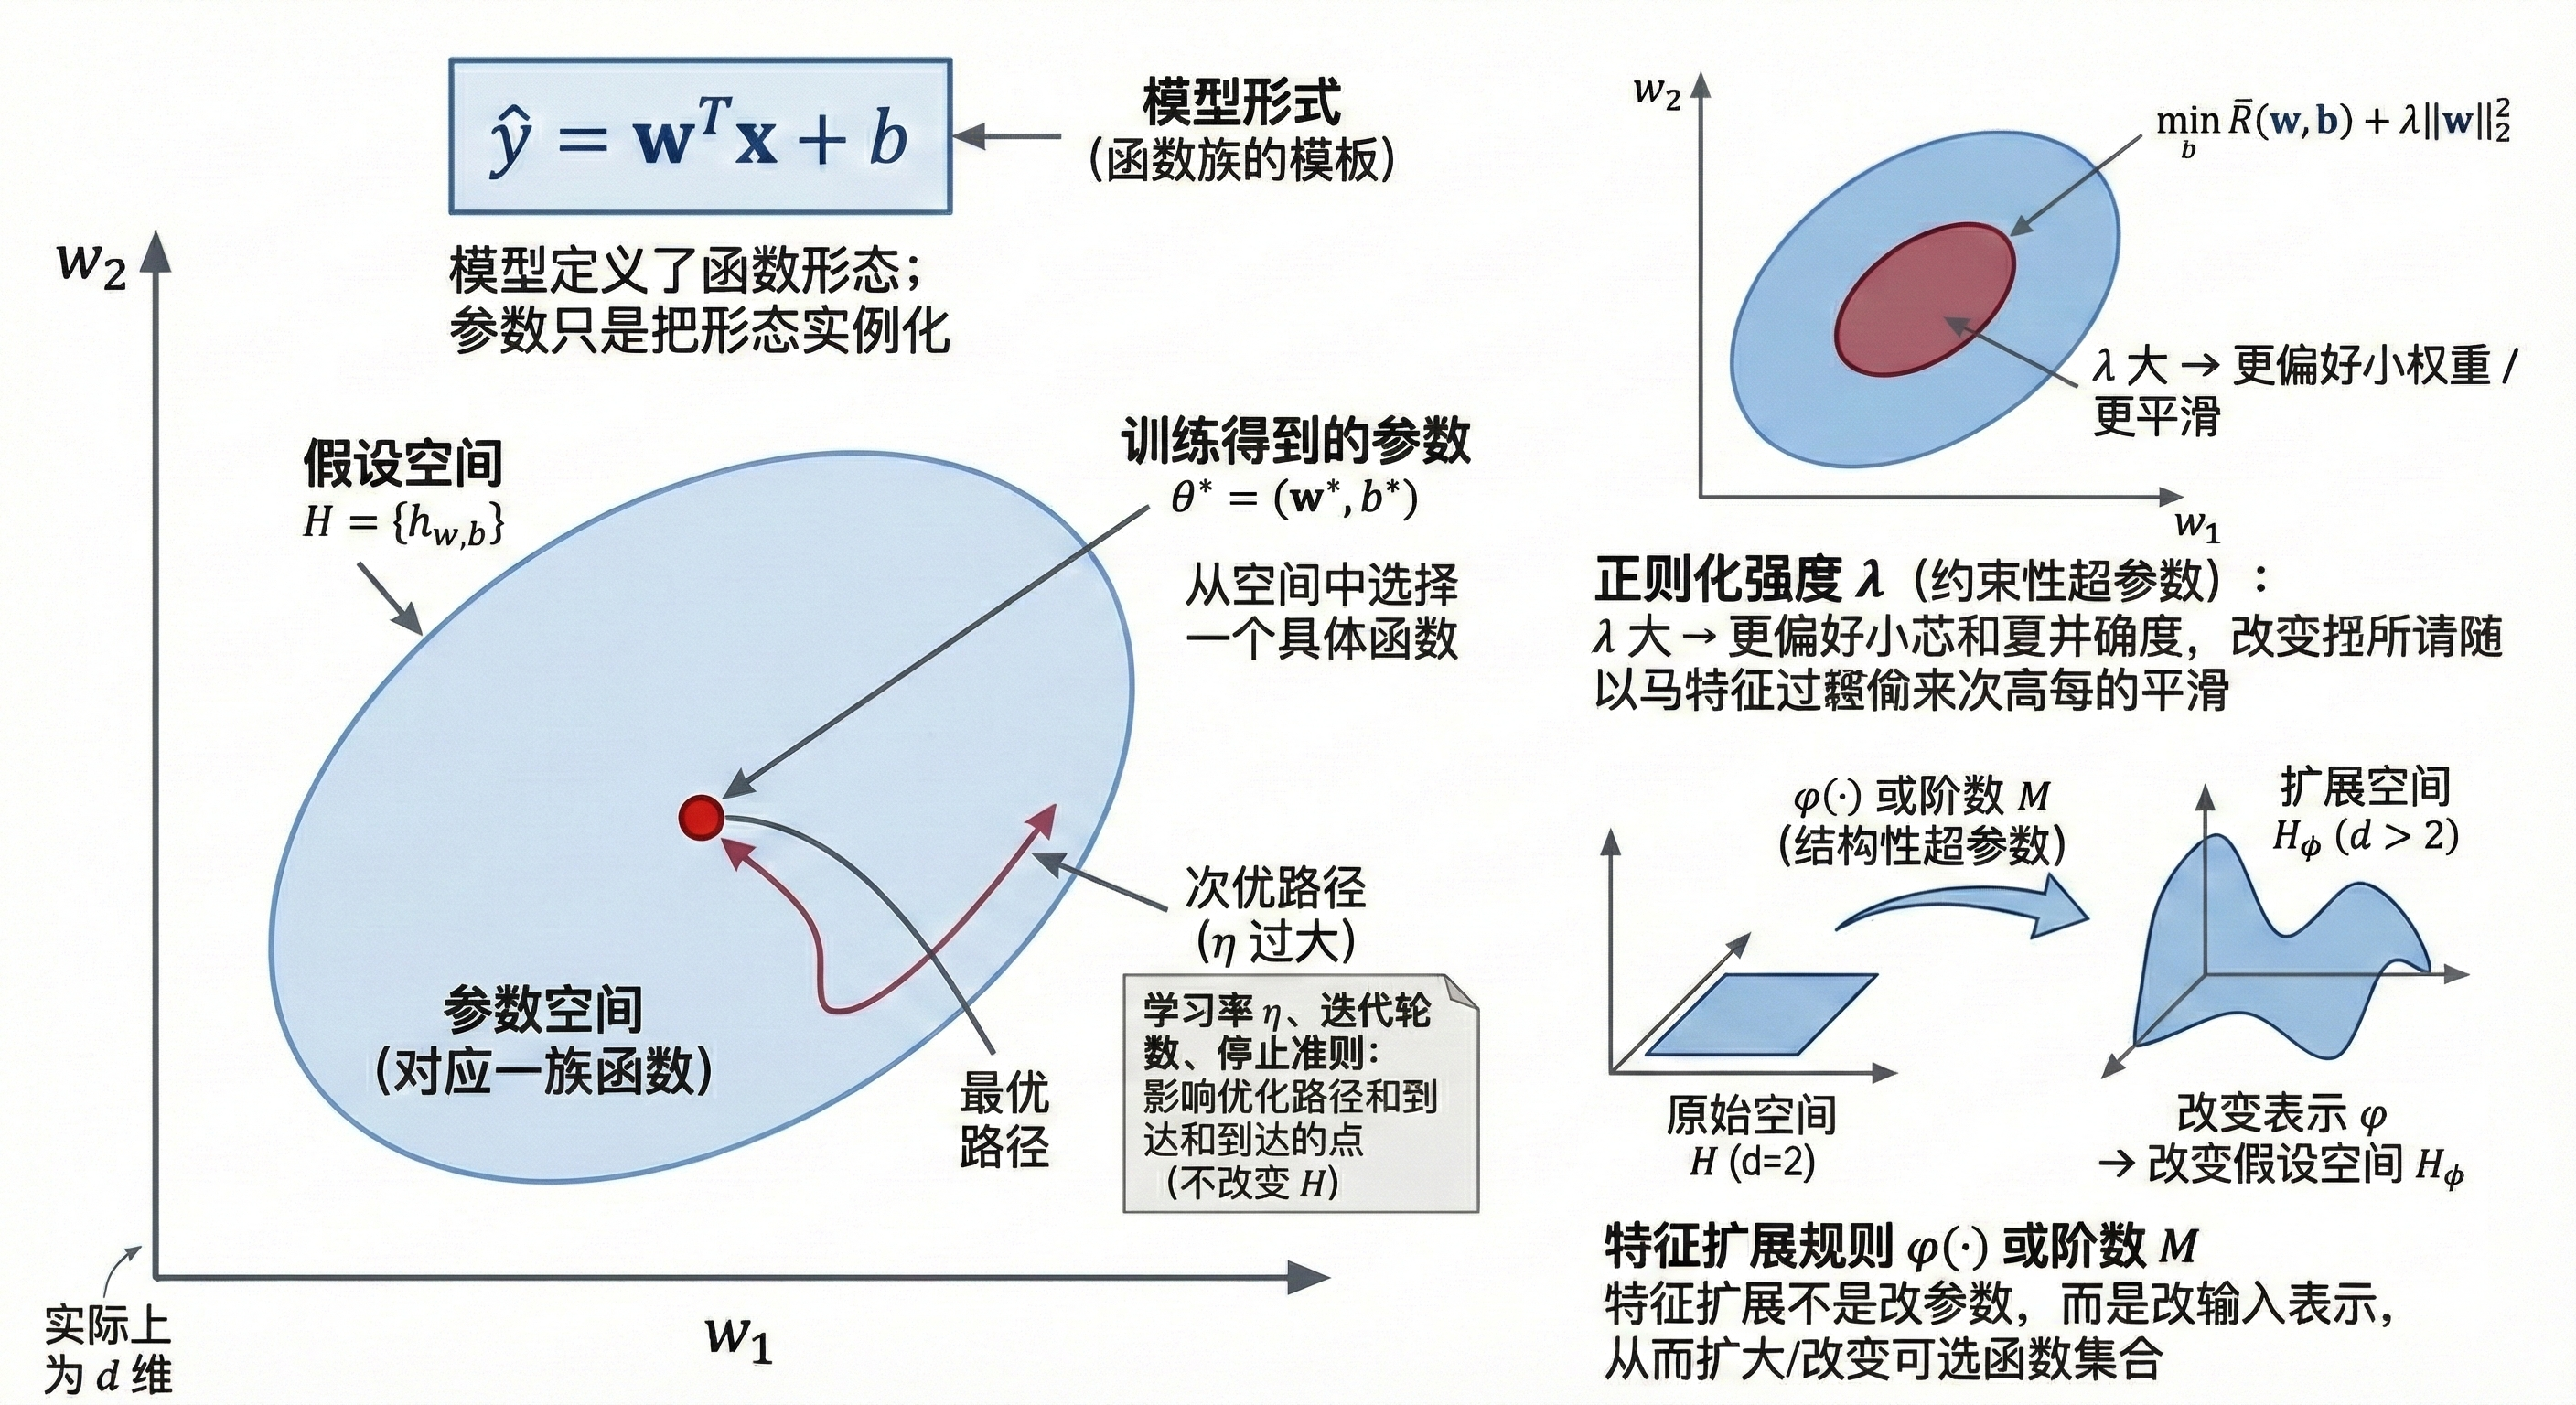
\includegraphics[width=0.8\textwidth]{figures/fig-3-3-1-model-concepts.png}
\caption{模型、假设空间、参数与超参数的关系示意图}
\label{fig:3-3-1-model-concepts}
\end{figure}

\noindent \textbf{1)模型}

\noindent 在机器学习语境中,模型更准确地指一族参数化函数,用来近似真实但未知的映射关系。在线性回归中,我们选用如下参数化形式
$\hat{y}=f(x;\theta)=w^\top x + b$,
其中 $w\in\mathbb{R}^d$ 为权重向量,$b\in\mathbb{R}$ 为偏置,$\theta=(w,b)$ 为模型参数集合。

\noindent 这一表达式的关键不在于给出某个具体预测值,而在于规定了预测函数必须属于仿射函数这一类。换言之,模型在此阶段只是定义了允许的函数形态,即线性叠加,而具体形态由参数决定。模型形式一旦确定,后续训练与评估都在这一形式的约束下展开。

\noindent 线性是相对于特征表示 $x$ 而言的。若对原始变量做非线性变换并将其作为新特征,例如 $\log(\text{距离})$、$\text{面积}^2$、$\text{面积}\times\text{学区}$ 等,模型仍保持对特征向量 $x$ 的线性,但在原始变量上可表现为非线性。因此,模型表达能力并非只由公式是否线性决定,还取决于特征表示的构造方式。严格地说,模型形式与特征表示共同决定了可表达的函数集合。

\noindent \textbf{2)表示与归纳偏置}

\noindent 任何学习算法都不可能在所有可能函数上有效搜索,因此必须通过模型形式与特征表示引入结构性约束。这种约束可视为归纳偏置,即在观察有限样本后,我们倾向于选择哪类函数作为解释数据的规律。

\noindent 在线性模型中,归纳偏置体现在,在给定表示 $x$ 下,输出随特征变化呈线性叠加,模型倾向于用各特征的加权贡献解释预测。这种偏置带来的直接后果是,当真实关系接近线性或可由合适特征变换线性化时,线性模型在样本较少、噪声存在的情况下往往更稳定。当真实关系强非线性且特征表示不足时,线性模型会出现系统性偏差,表现为欠拟合。

\noindent 归纳偏置并非主观任性,而是学习可行性的必要条件。如果不通过某种方式限制候选函数集合,就无法在有限数据下形成可推广的结论。

\noindent \textbf{3)假设与假设空间}

\noindent 在学习理论中,假设指某个候选预测函数,假设空间指学习算法允许选择的全部候选函数集合。对于线性模型
$\mathcal{H}=\{h_{w,b}(x)=w^\top x+b \mid w\in\mathbb{R}^d,\, b\in\mathbb{R}\}$。
这里每一组 $(w,b)$ 都定义了一个具体假设 $h_{w,b}$,而 $\mathcal{H}$ 是所有这类仿射函数的集合。

\noindent 这一形式化描述的意义在于,训练并不是创造一个函数,而是在 $\mathcal{H}$ 中选择一个函数。假设空间的大小与结构直接影响两类能力。一是可逼近能力,即是否包含足够接近真实规律的函数。二是可泛化能力,即在有限样本下是否容易被噪声误导。当 $\mathcal{H}$ 过小,模型即使训练充分也难以拟合主要规律。当 $\mathcal{H}$ 过大,模型可能在训练集上拟合得过好而对新样本不稳定。

\noindent 在线性模型里,$\mathcal{H}$ 的规模最直观地受特征维度 $d$ 影响。加入更多特征等价于扩大参数维度,进而扩大候选函数集合。但规模并不只等同于参数数量,还与特征之间的相关性、数据噪声、以及后续引入的约束如正则化共同决定。

\noindent \textbf{4)参数}

\noindent 参数是由训练过程直接从数据中估计的量。在线性模型中,参数就是 $(w,b)$。训练的目标是在给定数据集 $\mathcal{D}$ 与某个训练准则下,选出最合适的参数,从而确定最终使用的具体假设 $h_{w,b}$。

\noindent 为了把参数学习说得严谨,需要明确训练准则。以最常用的平方损失为例,经验风险为
$\hat{R}(w,b)=\frac{1}{n}\sum_{i=1}^n (y_i-(w^\top x_i+b))^2$。
参数学习就是求解
$(w^\ast,b^\ast)=\arg\min_{w,b}\ \hat{R}(w,b)$。
在此框架下,$(w^\ast,b^\ast)$ 是由数据驱动的结果,数据改变,最优参数一般也会改变。由此可以看到,参数的本质是,在既定的函数族与训练准则下,对具体函数进行实例化的自由度。

\noindent 参数还承担解释性角色。在不发生严重共线性且特征尺度可比的前提下,$w_j$ 反映了第 $j$ 个特征对预测的边际影响方向与强度。然而在实际数据中,特征相关性、尺度差异、以及特征工程引入的交互项常使单个权重的因果解释不成立,因此需要区分预测贡献意义与因果效应意义。

\noindent \textbf{5)超参数}

\noindent 超参数是不在一次参数拟合过程中由数据直接估计得到,而是由建模者预先设定或通过外层搜索选择的量。它们通常分为两类,结构性超参数与约束及过程性超参数。线性模型提供了非常清晰的例子。

\noindent \textbf{(1)约束性超参数:正则化强度 $\lambda$}

\noindent 在有限样本与噪声存在时,仅最小化经验风险可能导致模型对训练数据的偶然波动过度敏感。为控制有效复杂度,常在目标中加入正则项,得到正则化经验风险
$\hat{R}_\lambda(w,b)=\frac{1}{n}\sum_{i=1}^n (y_i-(w^\top x_i+b))^2+\lambda\Omega(w)$。
若取 $\Omega(w)=\|w\|_2^2$ 即岭回归,则
$(w^\ast_\lambda,b^\ast_\lambda)=\arg\min_{w,b}\ \frac{1}{n}\sum_{i=1}^n (y_i-(w^\top x_i+b))^2+\lambda\|w\|_2^2$。
此处 $\lambda\ge 0$ 就是典型超参数。它不属于模型参数向量 $(w,b)$,但它改变了优化问题本身,从而改变最终解的性质。直观上,$\lambda$ 越大,对大权重惩罚越强,模型被迫更平滑,对单个特征的极端依赖更少。$\lambda$ 越小,模型更强调拟合训练误差。严格地说,$\lambda$ 控制了解的偏差与方差权衡,增大 $\lambda$ 往往提高偏差、降低方差,反之亦然。

\noindent 需要强调,$\lambda$ 并不会在一次拟合过程中自动学出来。改变 $\lambda$ 通常意味着改变学习问题的定义,因此必须重新训练得到新的 $(w^\ast_\lambda,b^\ast_\lambda)$。这也是其作为超参数的决定性特征。

\noindent \textbf{(2)结构性超参数:特征扩展的阶数或规则}

\noindent 仍保持模型形式 $\hat{y}=w^\top x+b$,如果我们对原始输入做特征扩展,例如加入多项式项与交互项,则等价于改变输入表示 $\phi(\cdot)$,使用
$\hat{y}=w^\top \phi(x)+b$。
这里 $\phi(x)$ 的构造规则,例如扩展到几阶、多大范围的交互项、是否包含某些领域特征,决定了特征维度与表示能力,从而改变了假设空间
$\mathcal{H}_\phi=\{h_{w,b}(x)=w^\top \phi(x)+b\}$。
扩展阶数 $M$ 或特征生成规则不是通过一次训练直接估计得到的,它是对候选函数集合边界的设定,因此属于结构性超参数。$M$ 越大,$\phi(x)$ 越丰富,$\mathcal{H}_\phi$ 越大,表达能力增强,但在有限样本下过拟合风险也随之上升。反之,$M$ 太小则可能无法表达关键非线性结构。

\noindent \textbf{(3)训练过程超参数:学习率、迭代轮数与停止准则}

\noindent 即便在线性模型中,尤其采用迭代优化而非闭式解时,学习率、迭代步数、停止阈值等也属于超参数。它们不改变假设空间的定义,但会影响优化路径与收敛质量。学习率过大可能不收敛,过小则收敛缓慢并可能停在次优区域。停止策略则影响拟合到什么程度,从而间接影响泛化表现。

\noindent 综上,在线性模型这一例子里,参数 $(w,b)$ 是训练要直接估计的对象。超参数如 $\lambda$、特征扩展规则、学习率等,则决定了模型容量与训练机制。二者在职责上严格分离。参数学习回答在既定学习问题下取哪个具体函数,超参数选择回答学习问题该如何定义才更有利于泛化。

\noindent \textbf{三\quad 损失函数、目标函数与优化:训练到底在做什么}

\noindent 仍以房价预测为贯穿例子。设输入特征向量 $x \in \mathbb{R}^d$,真实价格 $y \in \mathbb{R}$。训练数据为
$\mathcal{D}=\{(x_i,y_i)\}_{i=1}^n$。
可以把它理解为 $n$ 条历史成交记录,每条记录是一套房子的信息与成交价配对样本。

\noindent \begin{figure}[htbp]
\centering
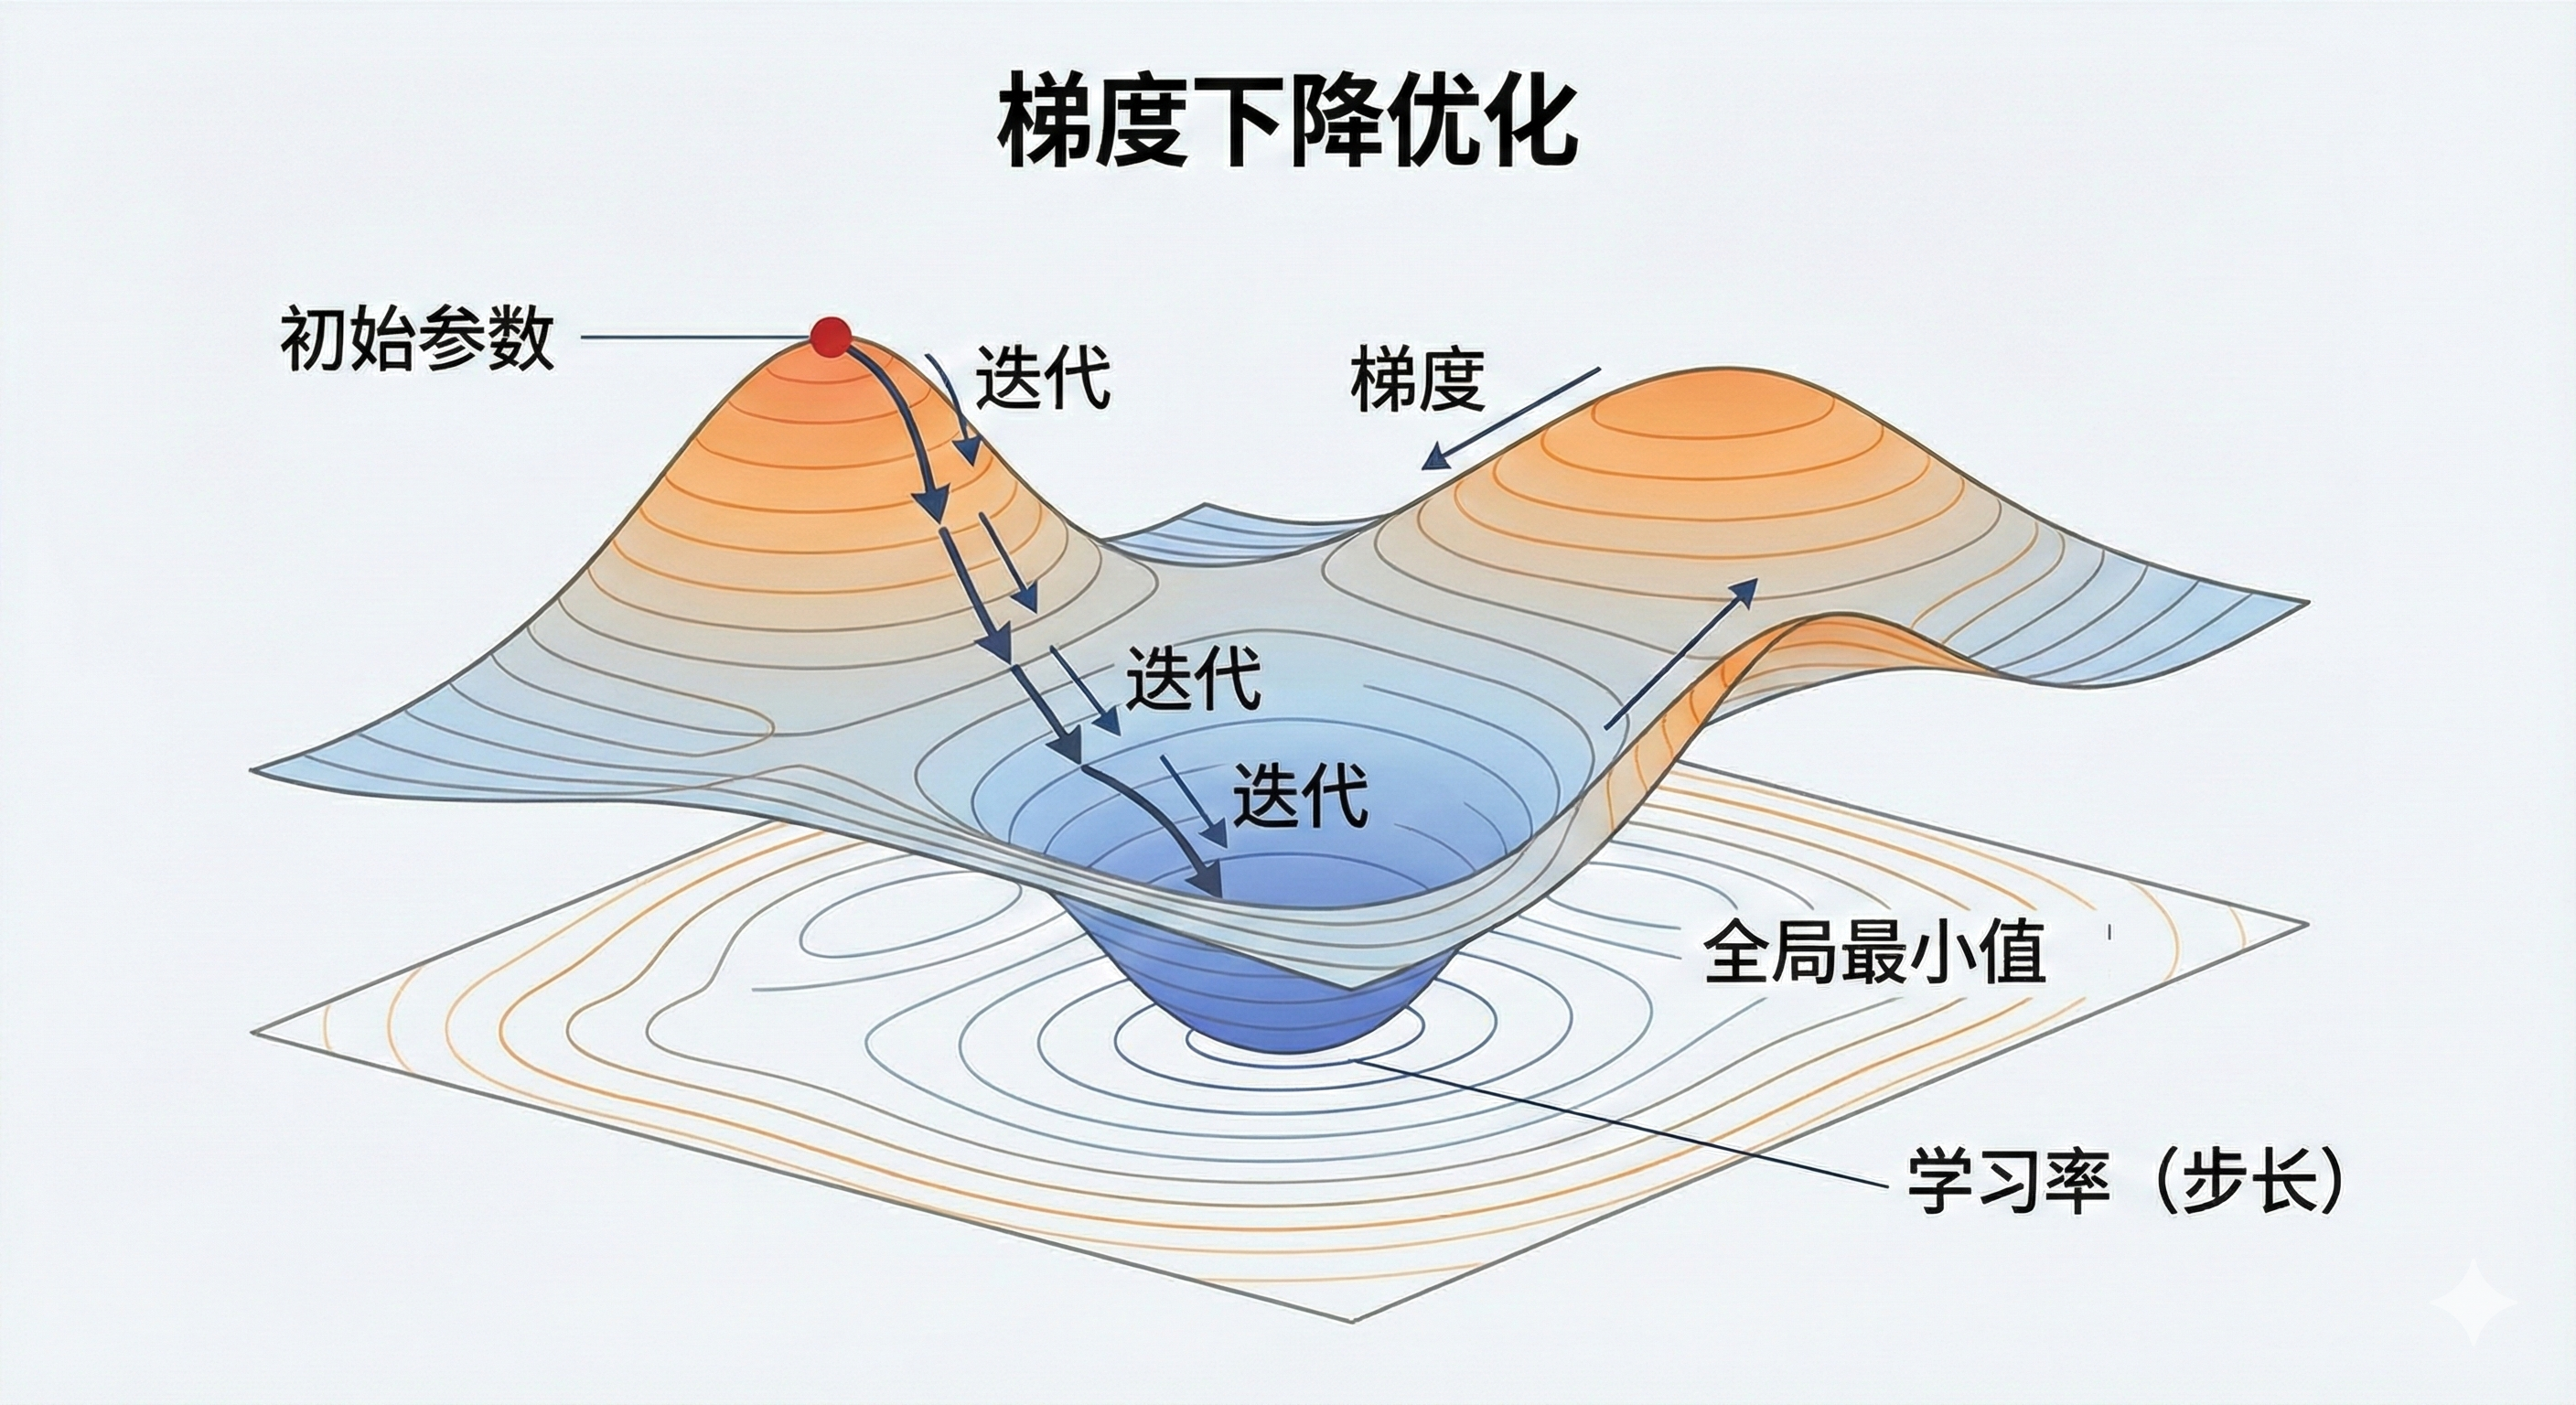
\includegraphics[width=0.75\textwidth]{figures/fig-3-3-3-loss-optimization.png}
\caption{\textbf{损失函数、目标函数与优化关系示意图}}
\label{fig:3-3-loss-optimization}
\end{figure}

\noindent \textbf{1)损失函数:把预测误差定义成一个可计算的数}

\noindent 损失函数衡量单个样本上的预测误差
$\ell\big(y,\hat{y}\big)=\ell\big(y,f(x;\theta)\big)$。
其作用是把预测和真实差多少压缩成一个数值,使训练过程能够据此比较不同参数下的好坏。

\noindent 回归任务中最常用的是平方损失
$\ell_{\text{sq}}(y,\hat{y})=(y-\hat{y})^2$。
误差越大,惩罚增长越快,平方会放大大误差,因此模型会倾向避免出现特别离谱的预测。

\noindent 另一个常见选择是绝对损失
$\ell_{1}(y,\hat{y})=\lvert y-\hat{y}\rvert$。
它对异常值更鲁棒,但目标函数不如平方损失平滑,优化实现通常更复杂。

\noindent \textbf{2)经验风险与目标函数:训练在最小化什么}

\noindent 训练的基本策略是让模型在训练集上的平均损失尽可能小。平均损失称为经验风险
$\hat{R}(\theta)=\frac{1}{n}\sum_{i=1}^n \ell\big(y_i,f(x_i;\theta)\big)$。
可以把它看成把每条样本的误差打分汇总后取平均,平均分越低,说明整体拟合越好。

\noindent 在本例中采用线性模型
$f(x;\theta)=w^\top x+b$,
并使用平方损失,则经验风险写为
$\hat{R}(w,b)=\frac{1}{n}\sum_{i=1}^n \big(y_i-(w^\top x_i+b)\big)^2$。
每套房子的误差是真实价减预测价,平方后求平均即得到训练集上的整体拟合误差。

\noindent 因此,训练对应一个明确的优化问题
$(w^\ast,b^\ast)=\arg\min_{w,b}\ \hat{R}(w,b)$。
训练完成后输出的是一组参数 $(w^\ast,b^\ast)$,也就是在训练集上使平均误差最小的那条线性预测规则。

\noindent \textbf{3)正则化:为什么目标函数常常不止拟合误差一项}

\noindent 若只追求训练误差最小,有限样本下容易过拟合。模型可能把训练数据中的偶然波动也当成规律。为提升稳定性,常在目标函数中加入正则项
$J(\theta)=\hat{R}(\theta)+\lambda\Omega(\theta)$。
这意味着训练不仅要求误差小,还要求模型不要过于复杂或极端。$\lambda$ 控制两者的权衡,$\lambda$ 越大越强调简单稳健,$\lambda$ 越小越强调贴合训练数据。

\noindent 岭回归即 L2 正则是回归中最常见的形式之一
$J(w,b)=\frac{1}{n}\sum_{i=1}^n \big(y_i-(w^\top x_i+b)\big)^2+\lambda\|w\|_2^2$。
$\|w\|_2^2$ 可理解为对权重总体规模的惩罚,它会抑制权重变得过大,从而减少模型对少数特征的过度依赖,使预测更稳定。

\noindent Lasso 即 L1 正则则写为
$J(w,b)=\frac{1}{n}\sum_{i=1}^n \big(y_i-(w^\top x_i+b)\big)^2+\lambda\|w\|_1$。
$\|w\|_1$ 倾向产生稀疏权重,很多权重变为 0,相当于自动筛掉部分特征,同时也意味着优化问题更不平滑,实现上更讲究技巧。

\noindent \textbf{4)优化:目标函数确定后,参数如何被求出来}

\noindent 目标函数 $J(\theta)$ 确定后,训练就变成数值优化,在参数空间中寻找使 $J(\theta)$ 最小的点。在线性回归加平方损失的场景下,该问题性质良好,既可以用闭式解,也可以用迭代法。在大规模训练中,迭代法更常用。

\noindent \textbf{(1)梯度下降:沿着下降最快的方向迭代}

\noindent 当 $J(\theta)$ 可微时,梯度 $\nabla_\theta J(\theta)$ 表示目标函数增大最快的方向,因此更新时取反方向
$\theta_{t+1}=\theta_t-\eta \nabla_\theta J(\theta_t)$。
每一步都沿着让目标变小最快的方向走一小步。学习率 $\eta$ 决定步长,过大可能震荡甚至发散,过小会收敛很慢。

\noindent 为看清更新在纠正什么,先定义残差
$r_i = y_i-(w^\top x_i+b)$。
它就是第 $i$ 个样本真实值减预测值的误差,正值表示预测偏低,负值表示预测偏高。

\noindent 在平方损失下,经验风险对参数的梯度为
$\nabla_w \hat{R}(w,b)=-\frac{2}{n}\sum_{i=1}^n r_i x_i,\quad
\frac{\partial \hat{R}(w,b)}{\partial b}=-\frac{2}{n}\sum_{i=1}^n r_i$。
权重 $w$ 的更新由残差与特征的相关性驱动,某个特征在系统性低估或高估时更相关,它对应的权重就会被相应上调或下调。偏置 $b$ 则根据整体残差的平均方向调整,总体低估就上调 $b$,总体高估就下调 $b$。

\noindent 若加入岭正则 $\lambda\|w\|_2^2$,梯度变为
$\nabla_w J(w,b)=-\frac{2}{n}\sum_{i=1}^n r_i x_i + 2\lambda w,\quad
\frac{\partial J(w,b)}{\partial b}=-\frac{2}{n}\sum_{i=1}^n r_i$。
额外项 $2\lambda w$ 会持续把权重往 0 拉回,从而抑制权重膨胀,提升模型稳定性。

\noindent \textbf{(2)批量、随机与小批量:每次用多少数据算梯度}

\noindent 批量梯度下降每次用全部 $n$ 条样本计算梯度,方向稳定,但单步计算开销大。随机梯度下降每次用 1 条样本近似梯度,更新频繁、单步很快,但方向噪声大,对学习率更敏感。小批量梯度下降每次用一小批样本,如 32 或 128,估计梯度,在速度与稳定性之间折中,是工程实践最常用的方式。

\noindent \textbf{5)学习率与停止:训练为何会跑偏或停得不合适}

\noindent 学习率 $\eta$ 决定每次纠错的力度。若 $\eta$ 过大,可能出现目标值震荡甚至上升,若过小,训练会极慢且在有限算力下难以达到足够好的解。实践中常配合学习率衰减、动量或自适应学习率方法以提高效率和稳定性。

\noindent 停止准则决定训练何时结束。对线性回归这类问题,可以用目标函数下降幅度很小或梯度足够小作为收敛信号。在更一般的学习任务中,还应结合验证集,当训练误差继续下降而验证误差不再下降甚至上升时,通常意味着过拟合正在发生,应考虑早停或增强正则化。

\noindent \textbf{四\quad 训练、验证与测试:为什么必须拆分数据}

\noindent 仍以房价预测为例。设数据集 $\mathcal{D}=\{(x_i,y_i)\}_{i=1}^n$,模型为 $\hat{y}=f(x;\theta)$,损失函数为 $\ell(y,\hat{y})$。上一节指出,训练阶段最小化的是训练数据上的平均损失即经验风险
$\hat{R}_{\mathcal{D}}(\theta)=\frac{1}{|\mathcal{D}|}\sum_{(x,y)\in \mathcal{D}}\ell\big(y,f(x;\theta)\big)$。
这一量反映的是模型对已见样本的拟合程度,但不能直接保证模型对未见样本同样可靠。训练、验证与测试的划分,正是为了解决拟合与泛化之间的天然张力。

\noindent \begin{figure}[htbp]
\centering
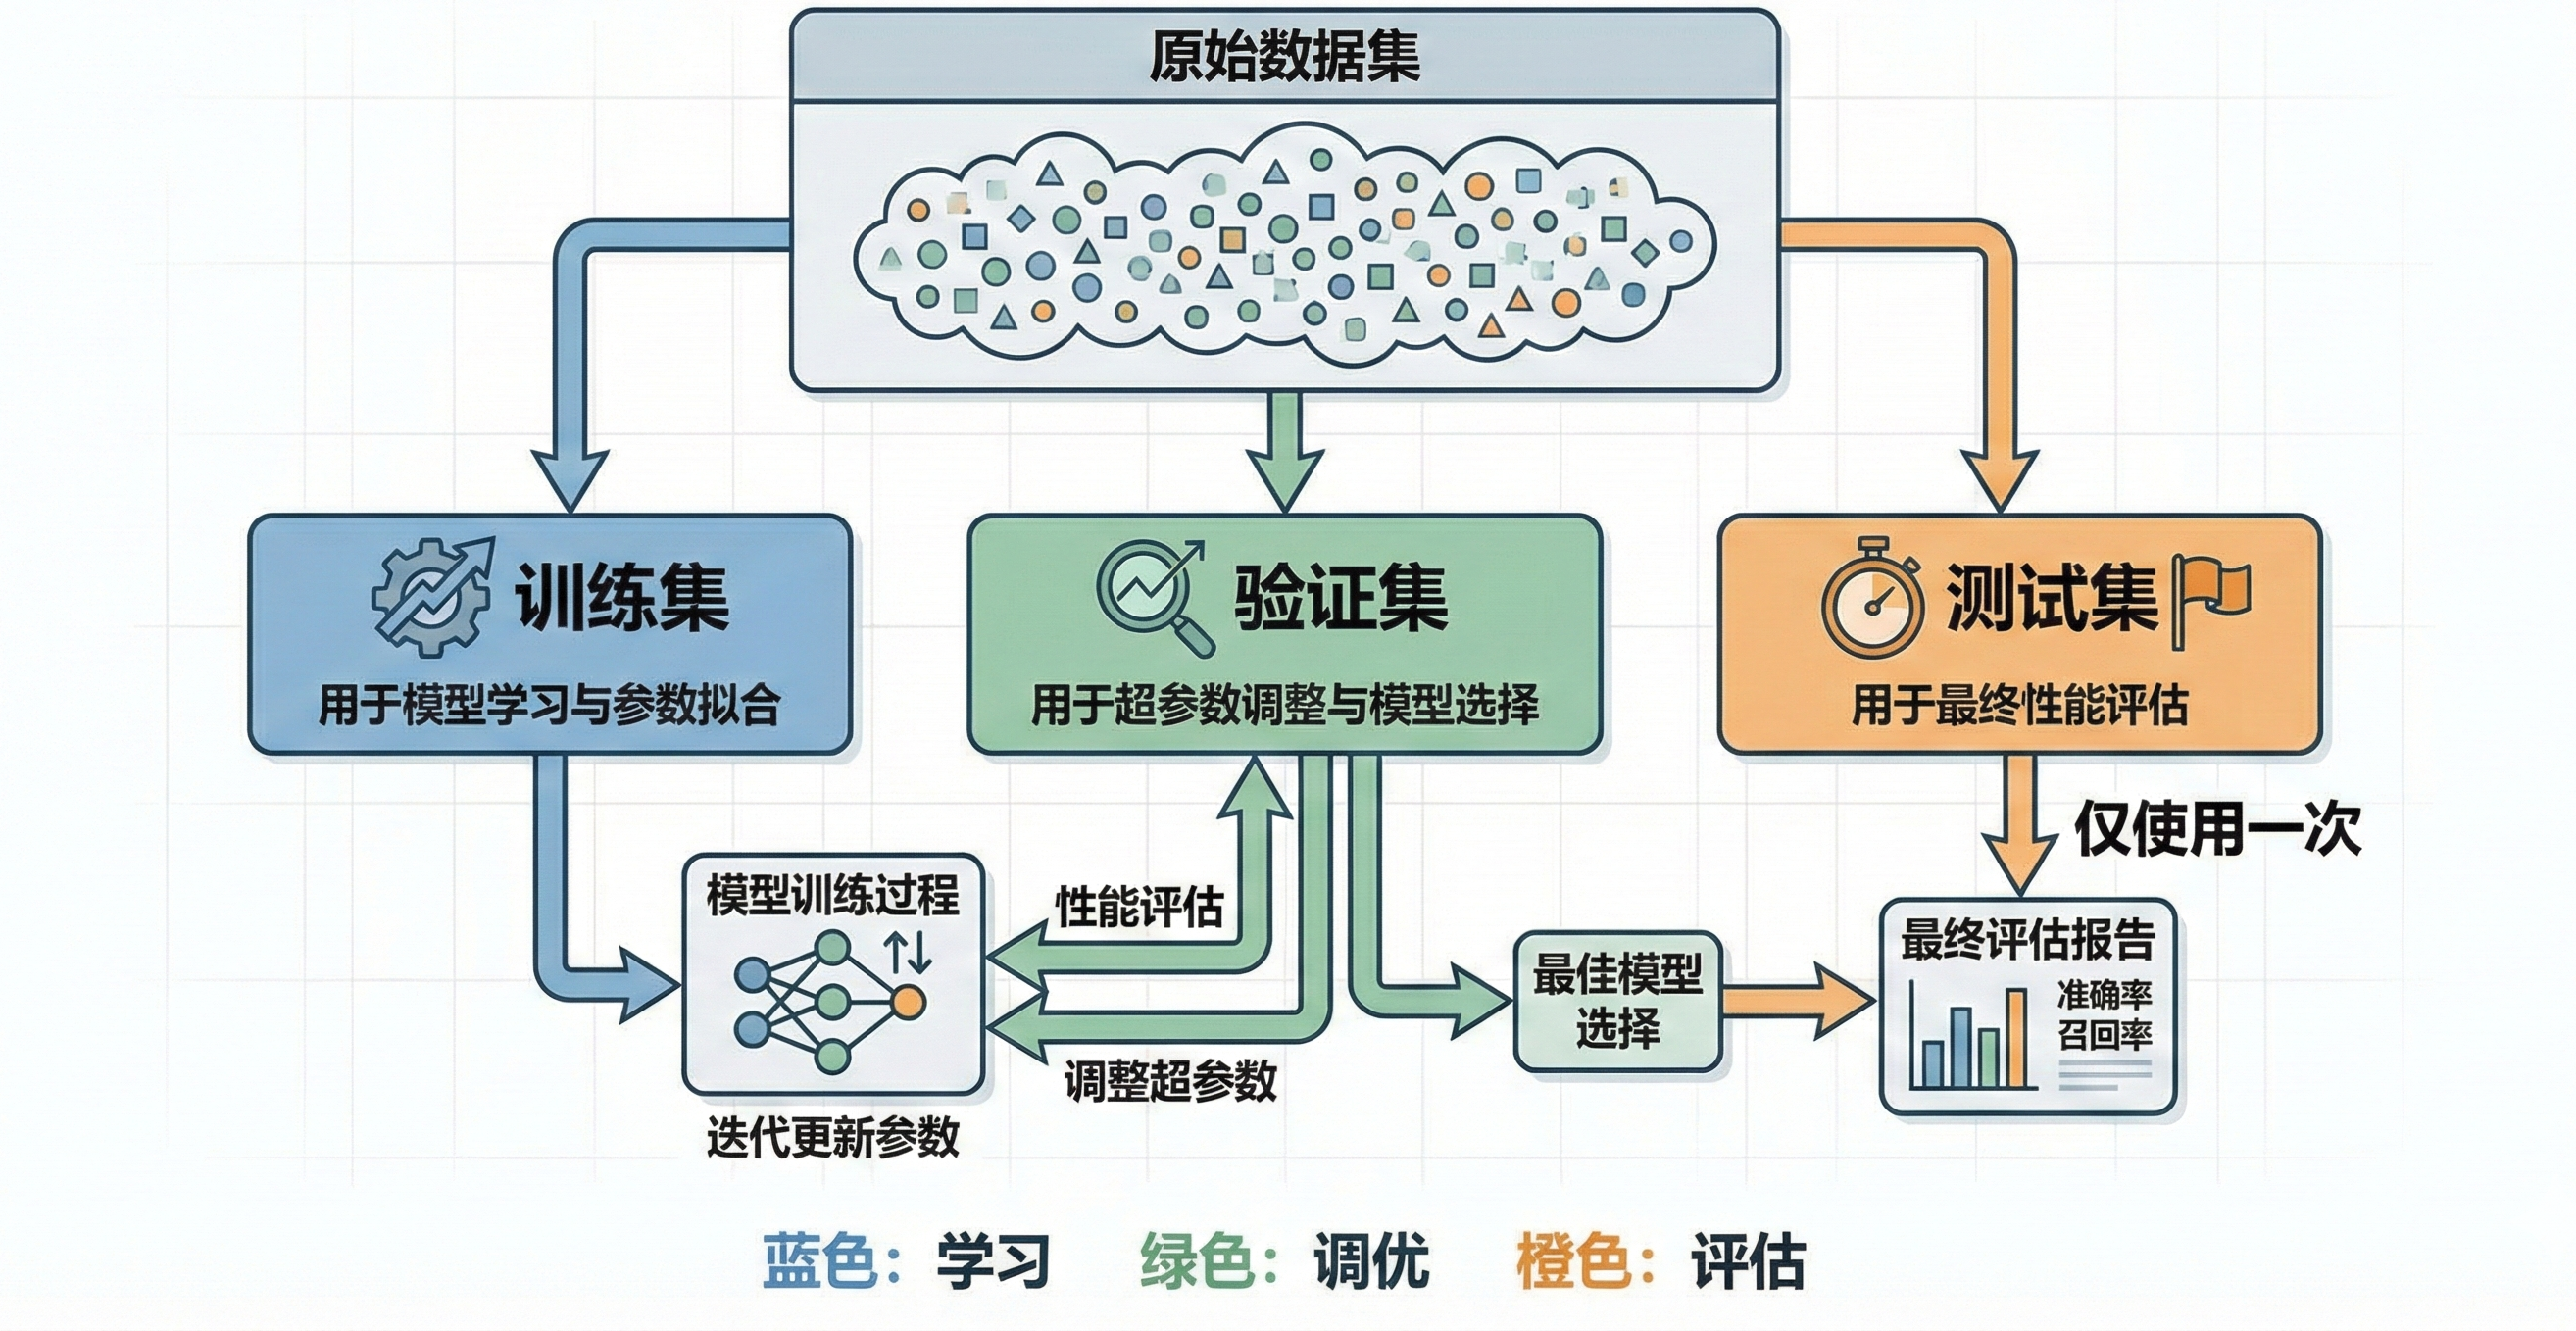
\includegraphics[width=0.75\textwidth]{figures/fig-3-3-4-train-val-test.png}
\caption{\textbf{训练、验证与测试数据划分关系示意图}}
\label{fig:3-3-4-train-val-test}
\end{figure}

\noindent \textbf{1)从训练误差到泛化误差:评估对象必须与目标一致}

\noindent 机器学习最终关心的是模型在未来数据上的表现,而不是在训练集上的表现。理想情况下,我们希望最小化真实数据分布 $P(x,y)$ 下的期望风险即泛化误差
$R(\theta)=\mathbb{E}_{(x,y)\sim P}\big[\ell\big(y,f(x;\theta)\big)\big]$。
由于 $P$ 不可直接获得,只能用样本近似。数据拆分的本质作用在于,用一份不参与训练的数据来近似评估 $R(\theta)$,并把这种评估结果用于模型选择与结论报告,从而避免训练误差下降被误读为未来表现变好。

\noindent \textbf{2)训练集、验证集与测试集:三种数据、三条不可混淆的职责}

\noindent 将数据拆分为互不重叠的三部分
$\mathcal{D}=\mathcal{D}_{\text{train}}\ \cup\ \mathcal{D}_{\text{val}}\ \cup\ \mathcal{D}_{\text{test}},\quad \text{两两不交}$。
更重要的是三者的权限边界,即哪一份数据可以影响哪些决策。

\noindent 训练集只负责学习参数 $\theta$,用于拟合模型参数
$\theta^\ast=\arg\min_{\theta}\ \hat{R}_{\mathcal{D}_{\text{train}}}(\theta)$。
训练集是唯一允许参与学习的数据。凡是被模型或预处理流程从数据中估计出来的内容,都必须限定在训练集内部完成。典型例子包括标准化所需的均值与方差、缺失值填充的统计量、类别编码映射、降维变换、特征选择规则等。原因并不复杂,这些步骤会改变输入表示或目标函数,从而影响最终学到的参数。它们一旦吸收了验证或测试的信息,就等价于把未见数据提前泄露给了训练过程。

\noindent 验证集只负责模型选择与调参。验证集不用于拟合参数,而用于在多种候选方案之间做选择。设超参数为 $\lambda$,例如正则化强度、特征扩展阶数、学习率策略等,通常流程是对每个候选 $\lambda$,先在训练集上训练得到 $\theta^\ast(\lambda)$,再在验证集上评估
$\lambda^\ast=\arg\min_{\lambda}\ \hat{R}_{\mathcal{D}_{\text{val}}}\big(\theta^\ast(\lambda)\big)$。
验证集的地位可以理解为外层裁判,它不参与学习,但决定学哪一种。在房价预测中,这对应一系列真实决策,正则化强度应取多大、是否加入某类交互特征、训练轮数与早停如何设置、采用 MAE 还是 RMSE 作为主要优化目标等。只要某个选择会影响最终模型形态,就应当由验证集或交叉验证来支撑,而不是由测试集来支撑。

\noindent 验证集还承担诊断功能。当训练误差持续下降而验证误差不再下降甚至上升时,通常意味着模型开始捕捉训练集中的偶然波动,泛化能力下降。此时应当调整模型复杂度、正则化或特征方案,而不是继续把训练误差压到更低。

\noindent 测试集只负责最终一次性报告,用于在模型方案确定之后做最终评估
$\widehat{\text{Perf}}=\text{Eval}\big(f(\cdot;\theta^\ast(\lambda^\ast)),\ \mathcal{D}_{\text{test}}\big)$。
测试集的关键原则是只评估,不决策。它不应参与任何选择过程,包括但不限于选择超参数、选择特征方案、比较不同模型、决定是否继续训练、决定是否更换损失函数或指标等。一旦测试集被用于反复试错,它就不再代表未见数据,评估结果会系统性偏乐观,最终导致对真实部署效果的错误预期。

\noindent \textbf{3)为什么不能用测试集调参:避免评估偏差与隐性过拟合}

\noindent 模型开发往往是迭代式的,你会反复尝试不同特征、不同正则、不同训练策略。若每次迭代都查看测试集表现并据此决定下一步方向,那么测试集事实上被纳入了模型选择过程,相当于对测试集进行外层拟合。结果是隐性过拟合,最终选出的方案可能只是对这份测试集适配得更好,并不保证对未来数据同样有效。

\noindent 因此,测试集应被视为事后检验。当且仅当你已经用训练集完成参数学习、用验证集完成模型选择之后,才用测试集给出一次性结论。这个结论才具有可复现性与解释力。

\noindent \textbf{4)交叉验证:用重复评估换取更稳定的模型选择}

\noindent 当数据量较小、样本波动较大,单次训练与验证划分可能带来较大的评估方差,模型选择容易受恰好怎么划分的影响。交叉验证通过多次划分与重复训练评估降低这种偶然性。以 $K$ 折交叉验证为例,将数据拆为 $K$ 份,每次取一份作为验证,其余作为训练,对同一超参数 $\lambda$ 得到 $K$ 个验证误差并求平均
$\widehat{R}_{\text{CV}}(\lambda)=\frac{1}{K}\sum_{k=1}^{K}\ \hat{R}_{\mathcal{D}^{(k)}}\big(\theta^{\ast(k)}(\lambda)\big)$。
交叉验证的直接收益是,模型优劣不再依赖单次划分的运气,而是由多次划分下的平均表现决定,从而更接近稳定的泛化估计。需要强调的是,交叉验证用于替代或增强验证集的角色,而不是替代测试集,测试集仍应保留为最终一次性评估。

\noindent \textbf{5)损失函数与评估指标:训练最小化的与业务关心的未必一致}

\noindent 训练时最小化的是损失函数构成的目标
$\min_{\theta}\ \hat{R}_{\mathcal{D}_{\text{train}}}(\theta)\quad \text{或 }+\lambda\Omega(\theta)$。
评估时关注的往往是业务可解释的指标,例如 MAE、RMSE、$R^2$,或在某个误差阈值内的命中率等。损失函数强调可优化性与训练稳定性,评估指标强调业务含义与决策相关性。二者可以不完全一致,但必须在设计上对齐。若训练目标与评估指标长期背离,模型可能训练得越来越好,但实际业务效果并不会同步改善。

\noindent \textbf{五\quad 泛化与误差}

\noindent 仍以房价预测为例。设真实价格为 $y$,模型预测为 $\hat{y}=f(x;\theta)$,损失函数为 $\ell(y,\hat{y})$。本节聚焦两件事。模型为何能在未见样本上保持有效,以及模型为何会出错、出错的来源与形态是什么。

\noindent \begin{figure}[htbp]
\centering
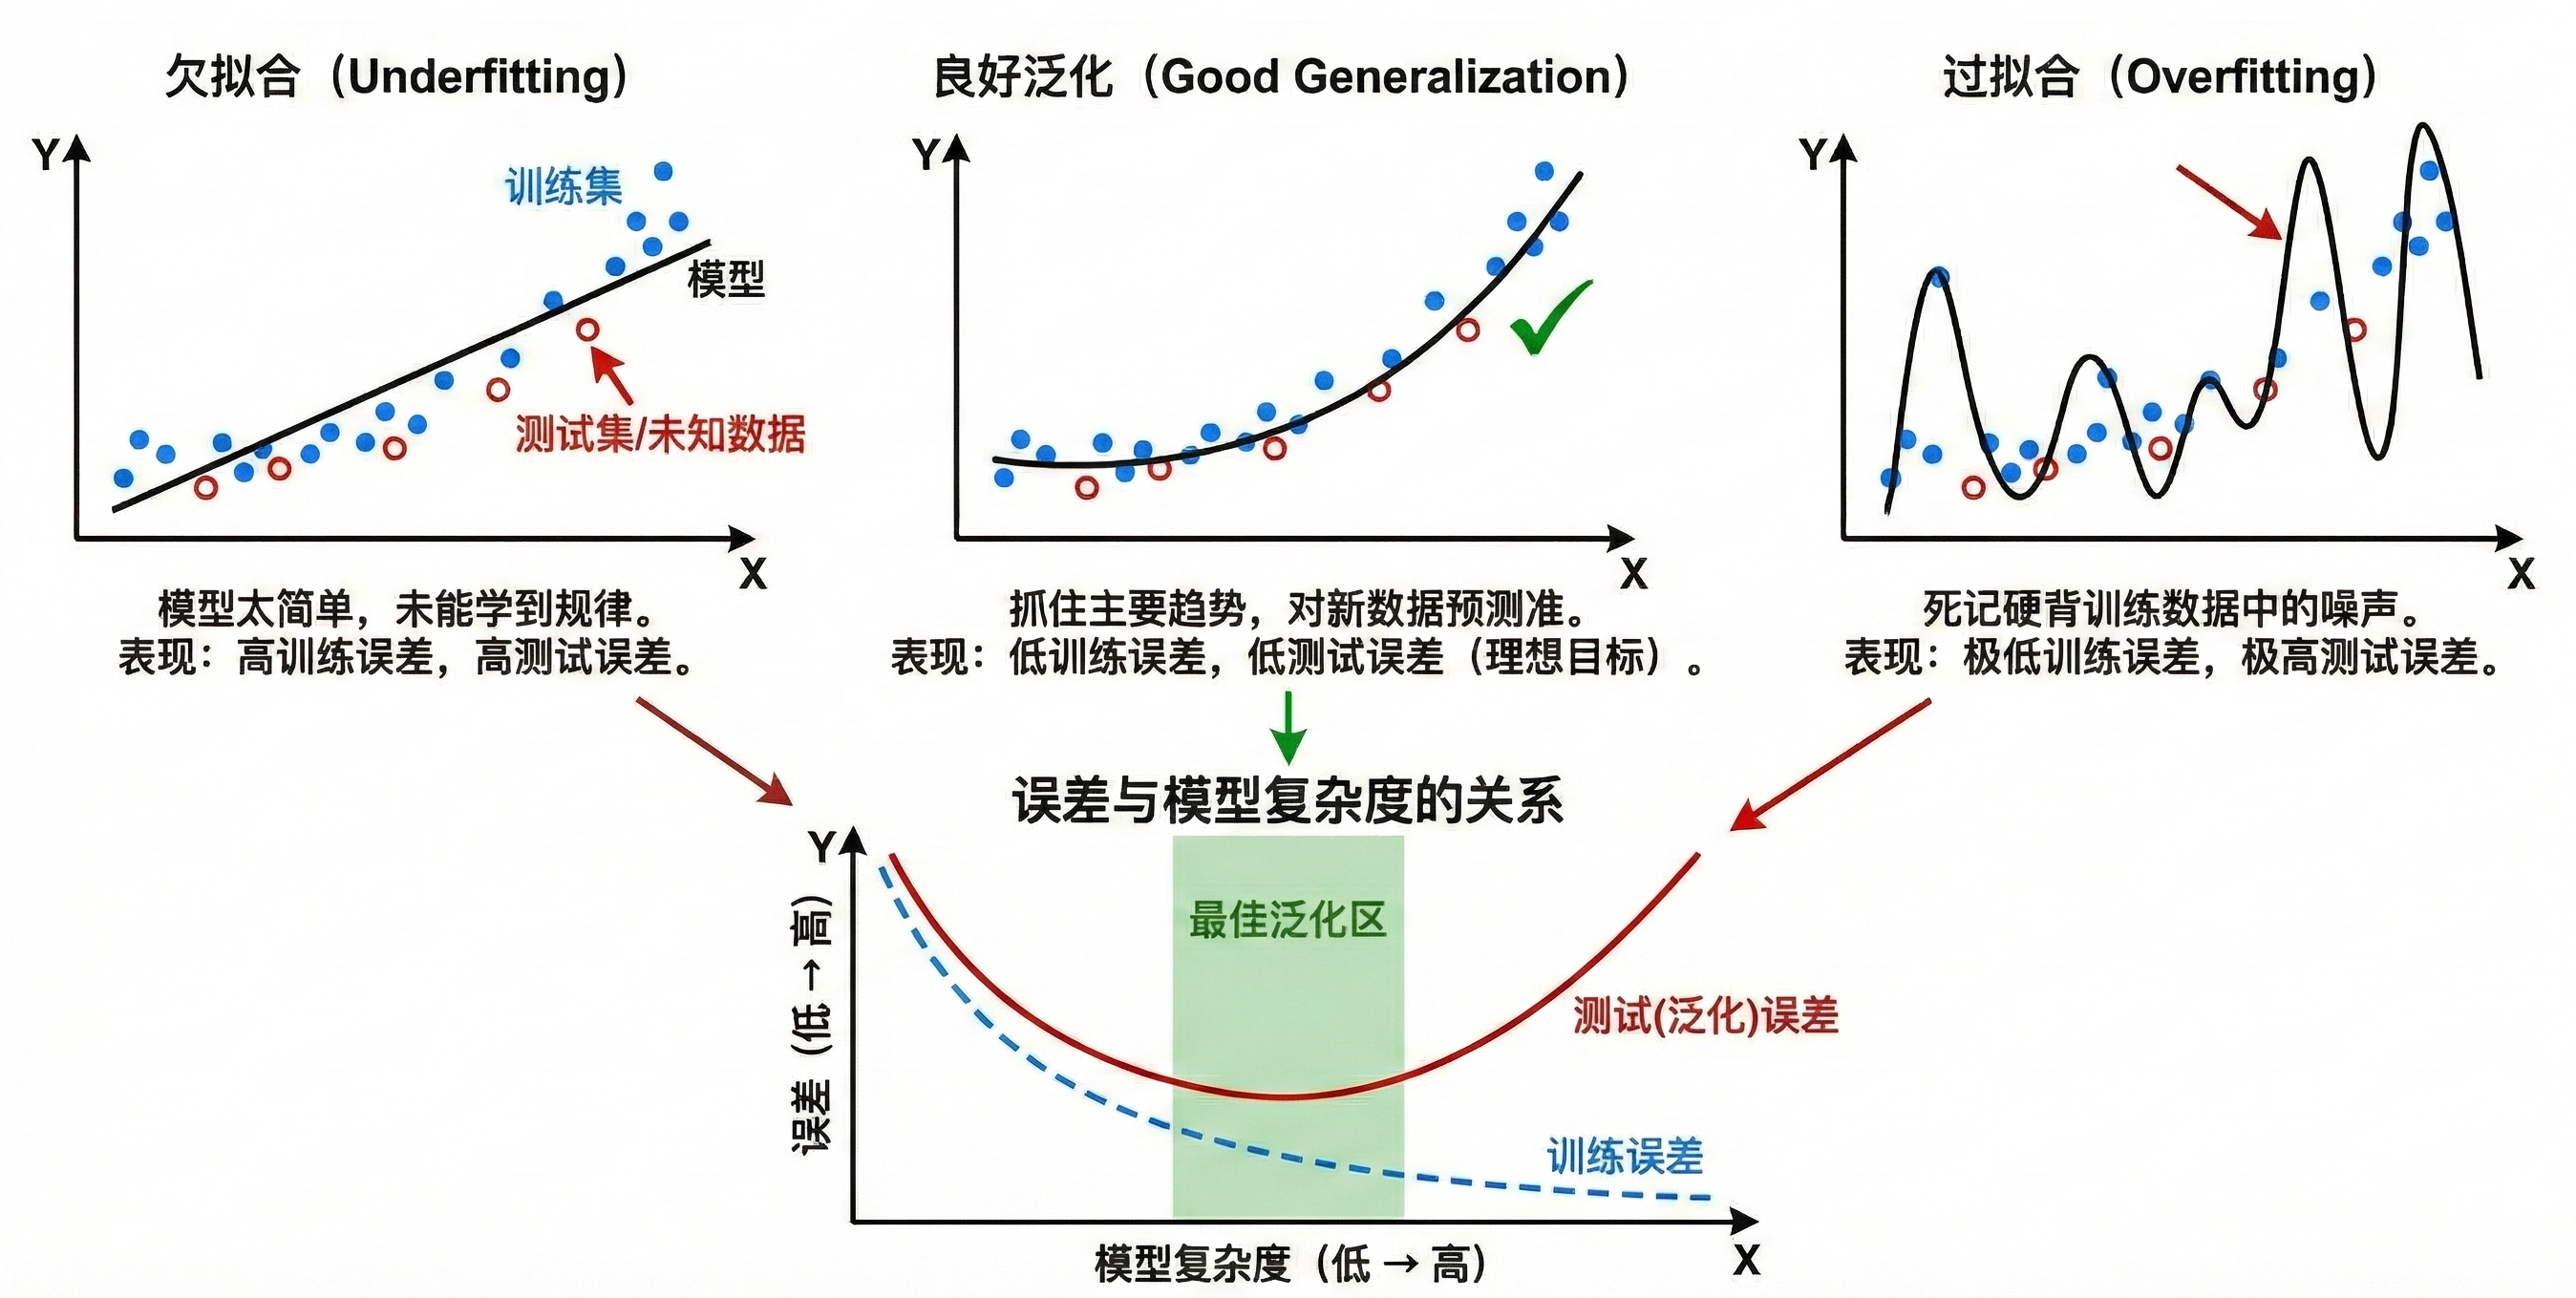
\includegraphics[width=0.75\textwidth]{figures/fig-3-3-5-generalization-error.png}
\caption{\textbf{泛化与误差关系示意图}}
\label{fig:3-3-5-generalization-error}
\end{figure}

\noindent \textbf{1)泛化:从训练集到未见数据}

\noindent 泛化指模型在未见样本上的表现能力。训练过程只保证模型对已见数据拟合得好,但最终目标是让模型在未来的新数据上同样可靠。实践中只能用一份不参与训练的数据,通常是验证集或测试集,来近似评估这种未来表现。之所以不用训练集评估泛化,是因为训练过程本身就是朝着降低训练集误差的方向更新参数,训练集上的损失更像是训练过程的内在产物,而不是对未来表现的独立估计。

\noindent \textbf{2)泛化间隙}

\noindent 令训练集与测试集上的经验风险分别为 $\hat{R}_{\text{train}}(\theta)$ 与 $\hat{R}_{\text{test}}(\theta)$。两者差值常用于刻画泛化间隙
$\Delta(\theta)=\hat{R}_{\text{test}}(\theta)-\hat{R}_{\text{train}}(\theta)$。
当 $\Delta(\theta)$ 明显为正且幅度较大时,意味着模型对训练样本的适配程度显著高于对未见样本的适配程度,通俗地说就是模型在训练数据上学得很像,但在新数据上像不起来。

\noindent 泛化间隙不是固定的模型属性,它是模型容量、数据规模、标签噪声、特征质量、正则化强度与优化细节共同作用的结果。同一个线性模型,在特征很多且噪声较大的场景中,与在特征精炼且样本充足的场景中,可能呈现完全不同的泛化表现。因此泛化诊断必须与具体数据及训练配置绑定,而不应简化为对某类算法的先验判断。

\noindent \textbf{3)误差的结构来源}

\noindent 对单个样本,预测误差可写为 $e(x)=y-f(x;\theta)$。从能否改进、如何改进的角度,误差来源通常分为三类。这个划分的价值在于它直接对应不同的工程处理策略。

\noindent 不可约误差即使存在最优规律,也可能因为测量误差、遗漏变量、信息不可得等原因,导致预测不可能做到完全准确。这部分误差不是通过换模型、调参或延长训练就能消除的。它决定了任务的上限,并提示模型之外的手段,如更高质量的采集、更关键的特征、更一致的标注规则,往往比更复杂的算法更能推动性能边界。

\noindent 系统性误差指模型在某些样本区域长期稳定地预测偏高或偏低,属于结构性偏差。这类误差常由模型形式表达能力不足、特征表示缺失关键信息、目标函数与业务目标不一致或数据中存在某些被忽略但强相关的条件变量触发。系统性误差的典型特征是方向一致、形态稳定。你会观察到某类房源被持续低估或高估,即便更换随机种子或小幅调参,偏差模式仍然存在。处理路径通常是增强表示能力、补齐关键特征或重新审视损失与指标是否对齐。

\noindent 不稳定误差指模型对训练数据扰动高度敏感,导致更换训练样本、改变采样顺序或初始化后,得到的参数明显不同,从而在未见样本上的表现波动较大。它常与有效信息不足而自由度过多有关。样本量不足、噪声较大、特征冗余严重、正则化不足、训练轮数过多都可能放大这种不稳定性。不稳定误差的经验信号包括训练误差可以很低但验证误差起伏大、不同训练轮次或不同随机种子下性能差异明显、某些特征权重出现不合理的大幅摇摆。处理路径往往是增加约束,如正则化与早停,降低有效自由度,如更少或更稳健的特征,提升数据有效性,如更多样本与更高标签一致性。

\noindent \textbf{4)欠拟合与过拟合}

\noindent 欠拟合与过拟合并不是抽象名词,而是训练误差与验证误差在数值上呈现出的两种典型组合形态。欠拟合表现为训练误差较高、验证误差也较高。这表明模型连训练数据中的主要规律都没有捕捉到。常见原因包括模型表达能力不足、特征信息不充分、正则化过强或训练未收敛。此时单纯加强正则化往往无助,关键在于提升可表达性与信息量。

\noindent 过拟合表现为训练误差很低而验证误差明显更高,即泛化间隙较大。这表明模型不仅学到了规律,也学到了训练数据中的偶然波动或噪声结构。常见原因包括有效自由度过大、正则化不足、训练轮数过多、标签噪声较大等。此时继续追求更低的训练误差通常会进一步恶化泛化,应转向控制复杂度与提升稳定性。

\noindent \textbf{5)结论性原则}

\noindent 第一,训练误差下降只说明模型更贴合训练集,不能单独作为模型学会规律的证据,泛化必须依赖验证或测试评估与误差类型分析来确认。第二,泛化问题本质上是有效信息量与有效自由度的匹配问题,信息不足时高自由度模型更容易不稳定,自由度不足时模型会出现稳定的系统性偏差。第三,误差分析优先回答错在什么类型,不可约、系统性还是不稳定,把误差类型识别清楚,后续改进才会从盲目试错变成可验证的工程迭代。

\subsubsection*{3.3.2\quad 监督学习}

\noindent \textbf{一\quad 监督学习要解决什么问题}

\noindent 监督学习处理的是有标准答案的学习。我们手里有一批样本,每个样本包含两部分,输入 $x$ 和对应的正确输出 $y$。把所有训练样本写成集合就是
$\mathcal{D}=\{(x_i,y_i)\}_{i=1}^n$,
其中 $x_i\in\mathbb{R}^d$ 是第 $i$ 个样本的 $d$ 维特征向量,$y_i\in\mathcal{Y}$ 是标签或目标值。监督学习要做的事,是从这些样本对里学到一个函数
$f(\cdot;\theta):\mathbb{R}^d\to \mathcal{Y}$,
使得当出现新的输入 $x$ 时,模型给出的预测 $\hat{y}=f(x;\theta)$ 尽可能接近真实的 $y$。

\noindent $x_i$ 像题目,$y_i$ 像标准答案。训练的目的不是把题目背下来,而是从题目与答案的对应关系中总结出规则。只要规则确实抓住了数据背后的稳定关系,那么在没见过的新题上也能做对,这就是泛化。

\noindent 根据输出空间 $\mathcal{Y}$ 的不同,监督学习最常见的两类任务是回归与分类。回归的输出是连续数值,$\mathcal{Y}\subseteq\mathbb{R}$,例如预测房价或温度。分类的输出是离散类别,$\mathcal{Y}$ 是有限集合,例如判断是否垃圾邮件或识别图像属于哪一类。两者本质一致,都是学习输入到输出的映射,只是输出的形式不同。

\noindent 为了让学习规则变成一个可执行的过程,需要三样东西,模型、损失、优化。模型给出如何从 $x$ 得到预测。损失函数把预测与真实的差异量化为一个数。优化算法通过调整参数让这个数变小。常见的训练目标写成
$\min_{\theta}\; J(\theta)=\frac{1}{n}\sum_{i=1}^n L\big(y_i,f(x_i;\theta)\big)$,
也就是让训练集上的平均损失尽量小。为了避免模型只在训练集上表现得像会了,而在新数据上不稳定,通常还会加上正则化项控制模型复杂度:
$\min_{\theta}\; \frac{1}{n}\sum_{i=1}^n L\big(y_i,f(x_i;\theta)\big)+\lambda\,\Omega(\theta)$.
可以把它理解为,一方面尽量把题做对,另一方面不要为了做对训练题而把规则弄得过于极端。

\noindent \begin{figure}[htbp]
\centering
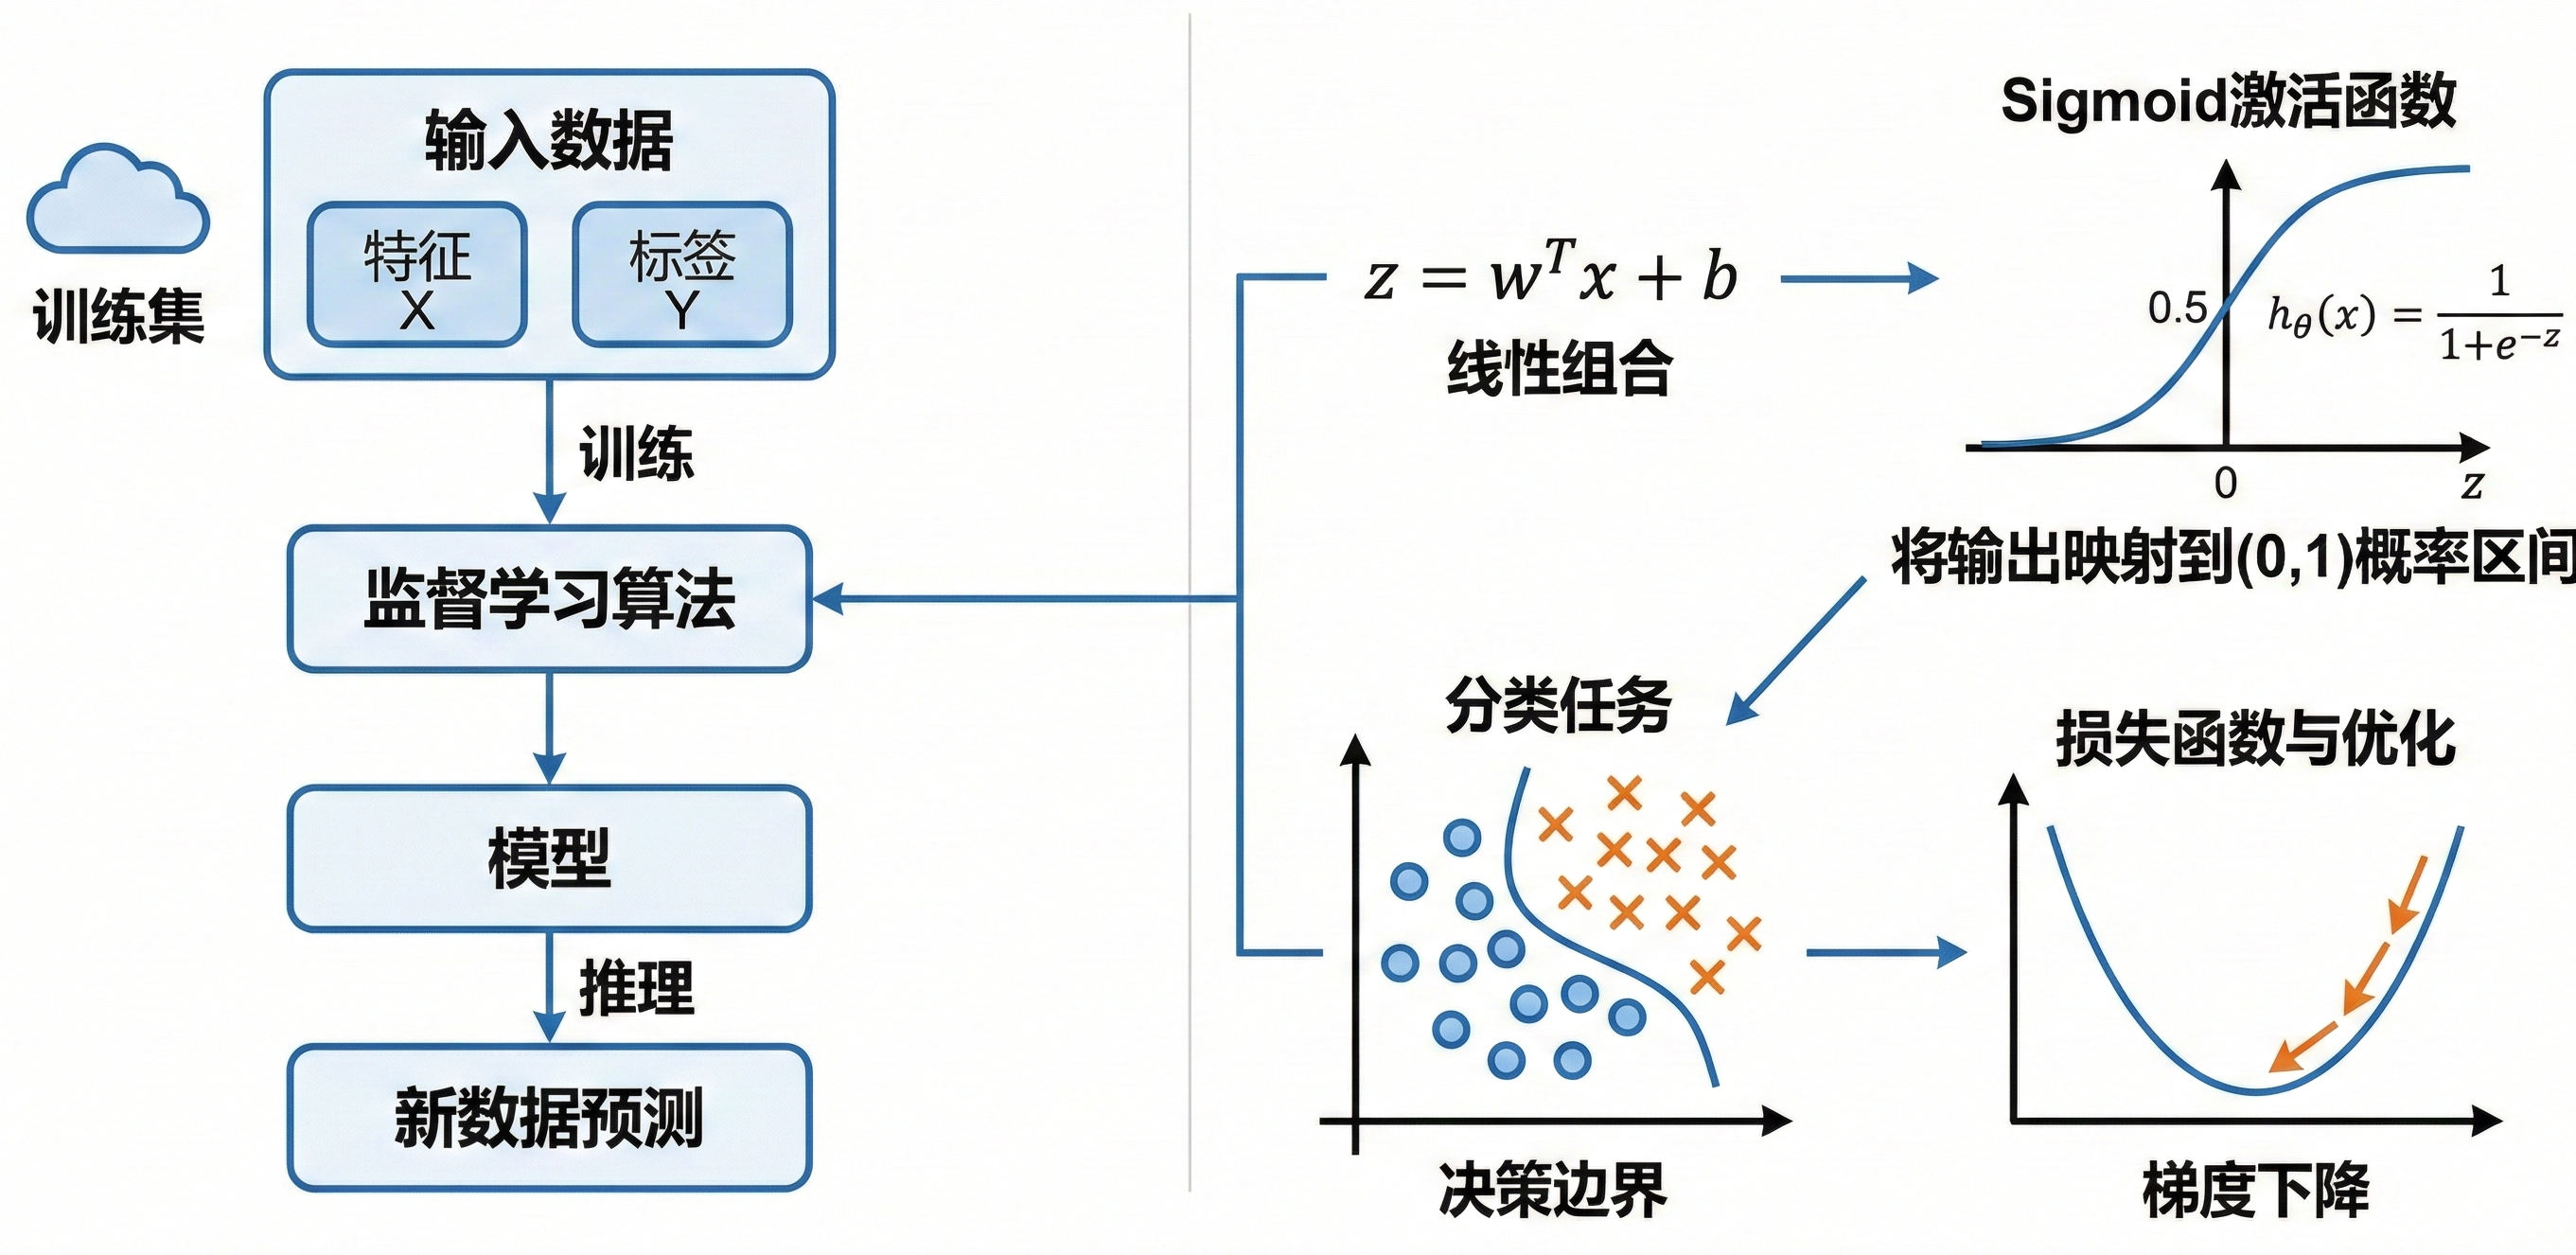
\includegraphics[width=0.75\textwidth]{figures/fig-3-3-2-supervised-learning.png}
\caption{\textbf{监督学习基本流程示意图}}
\label{fig:3-3-2-supervised-learning}
\end{figure}

\noindent \textbf{二\quad 一个经典的监督学习算法与计算实例}

\noindent 下面用逻辑回归贯穿监督学习的关键链条。逻辑回归是二分类的经典方法,标签取 $y\in\{0,1\}$。它既有清晰的概率解释,也能用非常简洁的数学式把训练过程写出来。

\noindent \textbf{1)模型如何给出预测}

\noindent 逻辑回归先给样本一个线性分数:
$z=w^\top x+b$,
然后把分数通过 Sigmoid 函数变成概率:
$p=\sigma(z)=\frac{1}{1+e^{-z}}$.
这里的 $p$ 可以直接解释为模型认为样本属于正类的概率,即
$P(y=1\mid x)=p,\qquad P(y=0\mid x)=1-p$.
$w$ 表示每个特征的重要程度。某个特征的权重为正,说明它越大越支持正类。权重为负则相反。线性部分把这些支持与反对的证据加总成一个分数 $z$,Sigmoid 再把这个分数压缩到 $0$ 到 $1$ 之间,得到可解释为概率的输出。

\noindent \textbf{2)用什么标准衡量预测好不好}

\noindent 逻辑回归通常用交叉熵损失:
$L(y,p)= -\big(y\log p+(1-y)\log(1-p)\big)$.
当 $y=1$ 时,损失变成 $-\log p$。如果模型给正类概率接近 $1$,损失接近 $0$。如果模型把概率给得很小,$-\log p$ 会变得很大,这等价于强烈惩罚明明是正类却极不自信的预测。
当 $y=0$ 时,损失是 $-\log(1-p)$,同理会惩罚明明是负类却给了很高正类概率的预测。

\noindent 在训练集上,目标就是让平均损失最小:
$J(w,b)=\frac{1}{n}\sum_{i=1}^n L(y_i,p_i),\quad p_i=\sigma(w^\top x_i+b)$.
为了抑制过拟合,常加入 L2 正则化:
$J_\lambda(w,b)=\frac{1}{n}\sum_{i=1}^n L(y_i,p_i)+\frac{\lambda}{2}\lVert w\rVert_2^2$.
这相当于鼓励权重不要过大,使模型的规则更平滑,不至于对某些特征的细小波动反应过度。

\noindent \textbf{3)训练一步到底做了什么}

\noindent 逻辑回归的一点优势是,它的参数更新可以写得非常透明。对单个样本 $(x,y)$,令
$p=\sigma(w^\top x+b)$,
那么交叉熵损失对参数的梯度是
$\frac{\partial L}{\partial w}=(p-y)x,\qquad \frac{\partial L}{\partial b}=p-y$.
如果用学习率 $\eta>0$ 做一次随机梯度下降更新,就得到
$w\leftarrow w-\eta(p-y)x,\qquad b\leftarrow b-\eta(p-y)$.
这组式子之所以直观,是因为核心只剩下一个量 $p-y$。它就是模型的偏差方向。当真实是 $1$ 但模型给的概率偏低时,$p-y<0$,更新会把 $w^\top x+b$ 往上推,从而让未来对相似样本给出更大的正类概率。当真实是 $0$ 但模型给的概率偏高时,$p-y>0$,更新会把分数往下拉,让正类概率下降。训练的迭代过程,就是不断用这种偏差去修正参数。

\noindent \textbf{4)一个可以手算的计算实例}

\noindent 取一个二维样本
$x=\begin{pmatrix}1\\2\end{pmatrix},\qquad y=1$.
设初始参数
$w=\begin{pmatrix}0\\0\end{pmatrix},\quad b=0,\quad \eta=0.1$.
先算分数
$z=w^\top x+b=0$,
于是
$p=\sigma(0)=0.5$.
这表示模型一开始没有任何偏好,只能给出 $50\%$ 的正类概率。

\noindent 接着计算 $p-y=0.5-1=-0.5$,并更新参数:
$w\leftarrow 0-0.1(-0.5)\begin{pmatrix}1\\2\end{pmatrix}
=\begin{pmatrix}0.05\\0.10\end{pmatrix},\qquad
b\leftarrow 0-0.1(-0.5)=0.05$.
再用更新后的参数对同一个 $x$ 计算一次:
$z'=(0.05,0.10)\cdot(1,2)+0.05=0.30$,
$p'=\sigma(0.30)=\frac{1}{1+e^{-0.30}}\approx 0.574$.
只更新一步,模型对这个正类样本的预测概率就从 $0.5$ 提升到了约 $0.574$,方向是正确的。把这种更新在大量样本上重复进行,模型会逐渐学到一组权重 $w$ 与偏置 $b$,使得不同特征组合对应的概率输出与标签规律一致,并且在新样本上也能保持稳定表现。

\noindent 这一例子把监督学习的闭环压缩成了可计算的形式。模型给出概率 $p$,标签提供目标 $y$,二者差异 $p-y$ 形成更新信号,更新信号推动参数改变,参数改变又影响下一次预测。理解了这条闭环,监督学习的其他算法,如线性回归、SVM、神经网络等,在结构上都可以看作同一思想的不同实现。

\noindent \textbf{5)代码实现}

\noindent 下面用Python代码实现上述逻辑回归的训练过程。这段代码与手算实例完全对应,展示了从初始化、预测、计算梯度到更新参数的完整流程。

\begin{lstlisting}[language=Python, caption={逻辑回归单步更新的Python实现}]
import numpy as np

# Sigmoid函数:将分数压缩到(0,1)区间
def sigmoid(z):
    return 1 / (1 + np.exp(-z))

# 定义样本和标签(对应手算实例)
x = np.array([1, 2])    # 输入特征
y = 1                   # 真实标签(正类)

# 初始化参数
w = np.array([0.0, 0.0])  # 权重向量
b = 0.0                   # 偏置
eta = 0.1                 # 学习率

# 第一步:预测
z = np.dot(w, x) + b      # 计算线性分数
p = sigmoid(z)            # 转换为概率
print(f"初始预测概率: {p:.3f}")  # 输出: 0.500

# 第二步:计算梯度
# 梯度 = (预测值 - 真实值) * 特征
gradient_w = (p - y) * x   # 对w的梯度
gradient_b = (p - y)       # 对b的梯度

# 第三步:更新参数
w = w - eta * gradient_w   # 更新权重
b = b - eta * gradient_b   # 更新偏置

print(f"更新后的权重: {w}")
print(f"更新后的偏置: {b:.3f}")

# 用新参数再次预测
z_new = np.dot(w, x) + b
p_new = sigmoid(z_new)
print(f"更新后预测概率: {p_new:.3f}")  # 输出: 0.574
\end{lstlisting}

\subsubsection*{3.3.3\quad 无监督学习}

\noindent \textbf{一\quad 无监督学习要解决什么问题}

\noindent 无监督学习面对的数据通常只有输入,没有对应的标准答案。形式上,给定数据集
$\mathcal{D}=\{x_i\}_{i=1}^n,\qquad x_i\in\mathbb{R}^d,$
我们希望从这些样本本身出发,提取数据的结构、规律或表示,而不是学习一个"从 $x$ 到 $y$"的映射函数。监督学习像是"有答案的练习册",无监督学习更像是"把一堆材料摆在面前,要求你自己归纳出它们的组织方式"。

\noindent 无监督学习的目标可以有多种等价表述。常见的一类是发现结构,例如把样本自动分组、识别数据中存在的模式或簇;另一类是学习表示,例如把高维数据压缩到低维但尽量保留关键信息,从而获得更紧凑、更有解释力或更利于下游任务的特征;还有一类是分布建模,即用概率模型刻画数据是如何生成的,从而能够估计密度、识别异常,甚至生成与数据分布一致的新样本。

\noindent 与监督学习相比,无监督学习最关键的差异在于训练信号来自"数据自身"。因此,问题的定义往往更依赖建模假设:你需要明确你认为数据里应该存在什么样的结构,或你希望保留什么样的信息。换句话说,无监督学习通常不是在问"预测对不对",而是在问"用某种结构或表示去解释数据是否合理"。

\noindent \begin{figure}[htbp]
\centering
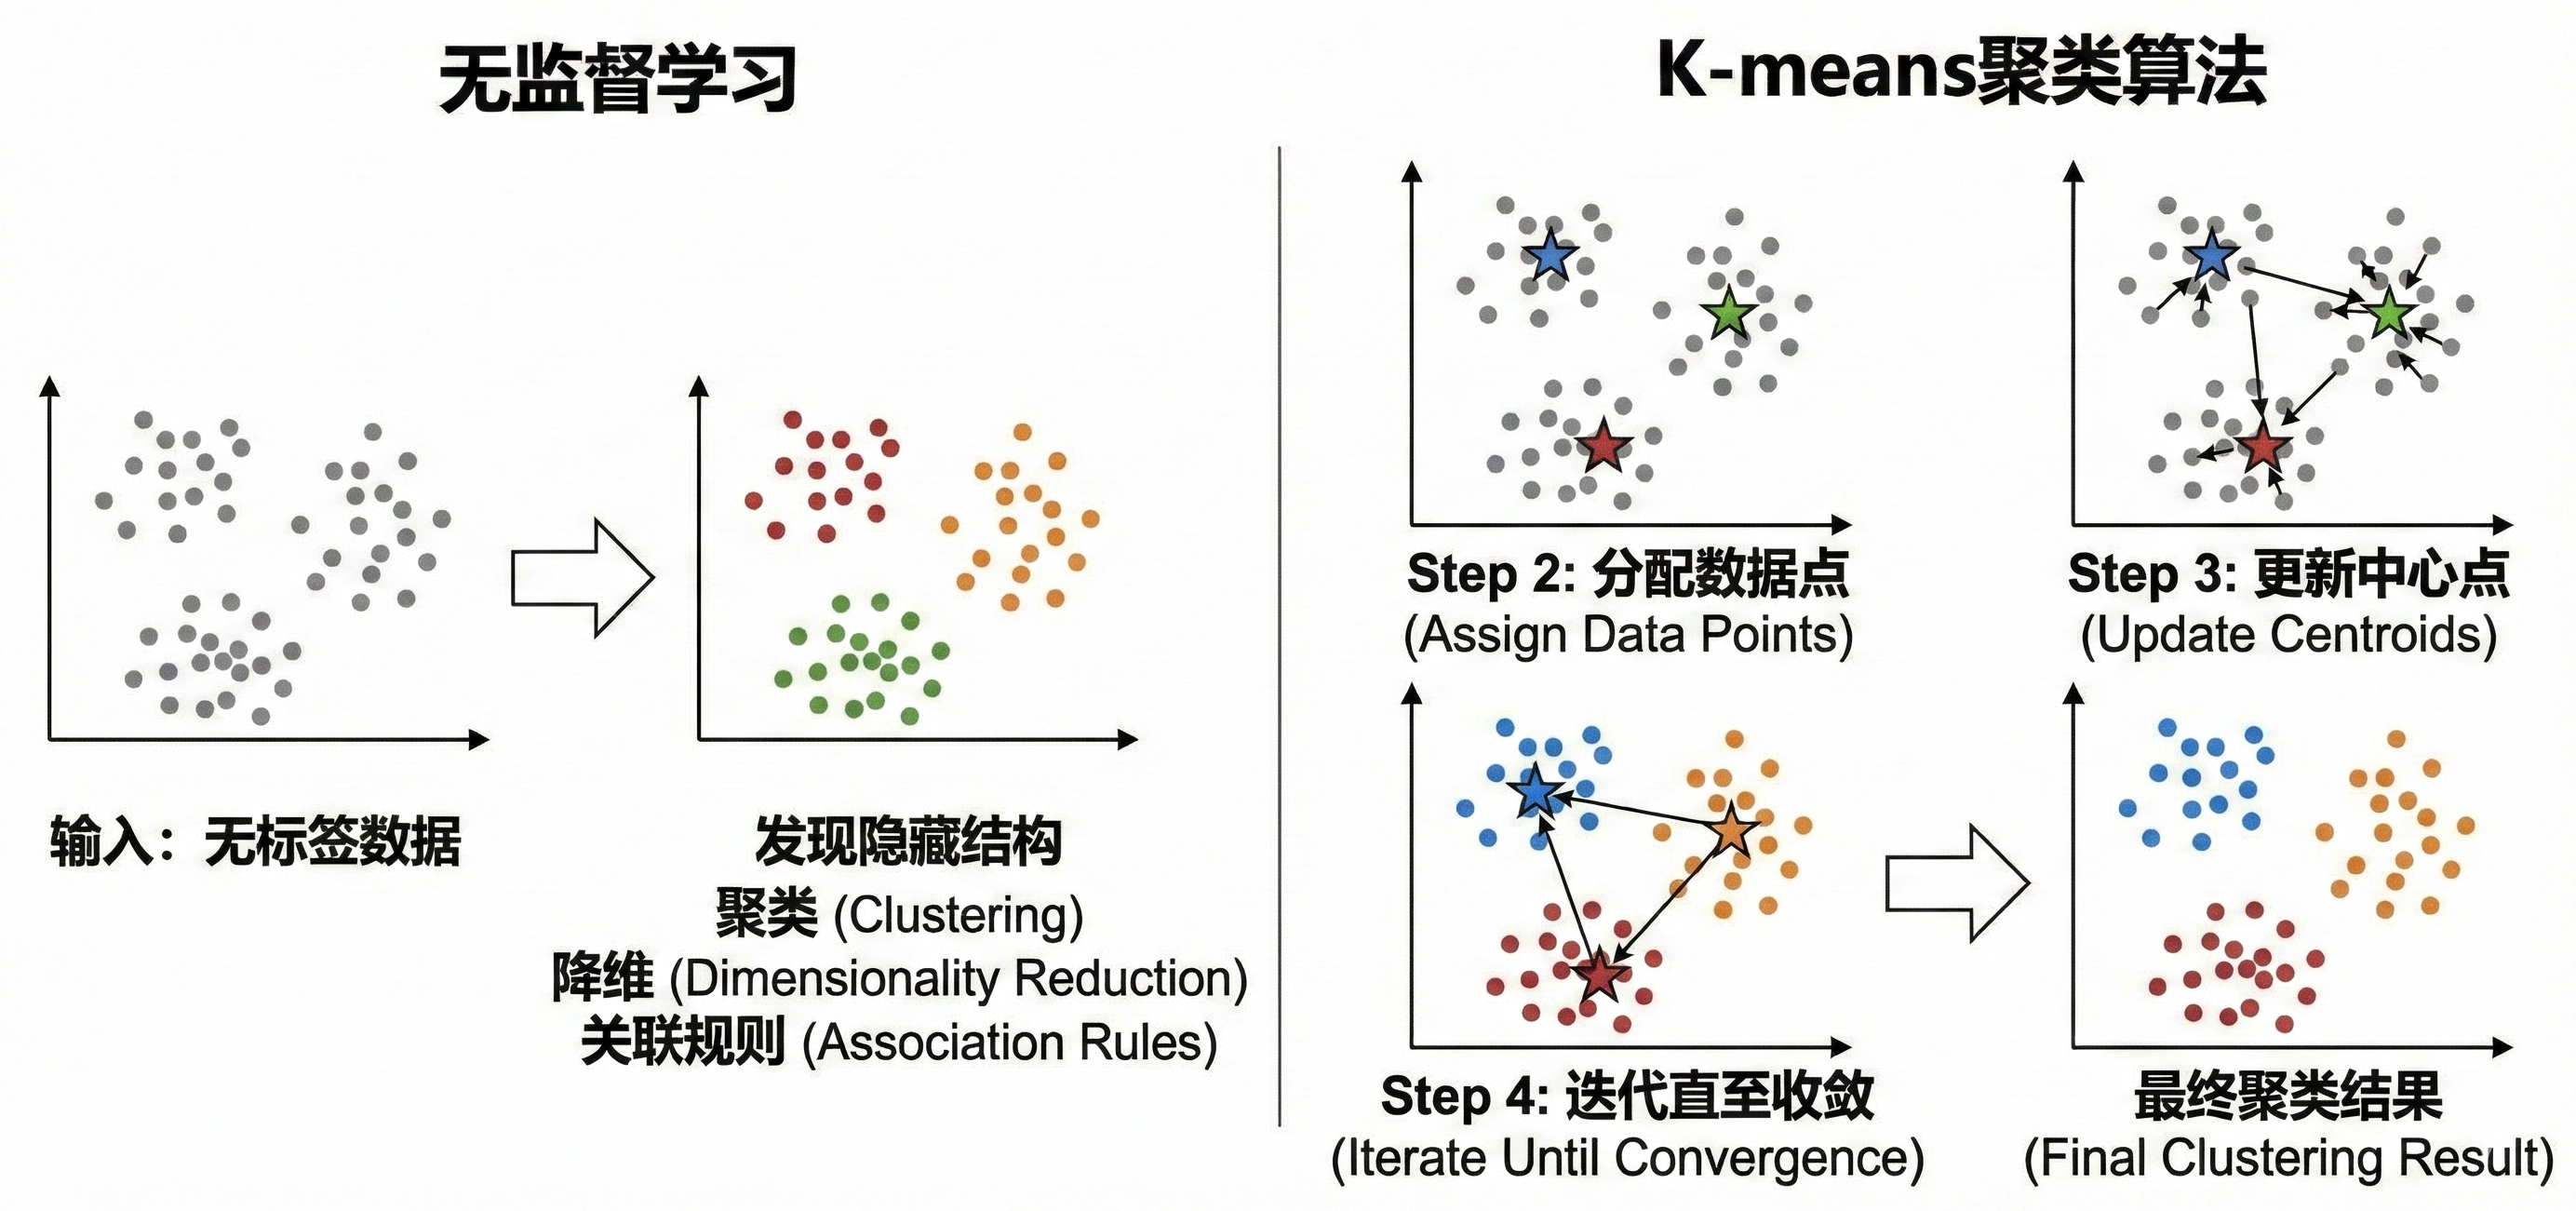
\includegraphics[width=0.75\textwidth]{figures/fig-3-3-3-unsupervised-learning.png}
\caption{\textbf{无监督学习基本流程示意图}}
\label{fig:3-3-3-unsupervised-learning}
\end{figure}

\noindent \textbf{二\quad 一个经典的无监督学习算法与计算实例}

\noindent 为了把无监督学习的数学对象讲清楚,下面以 K-means 聚类作为经典算法示例。聚类的目标是把样本分成若干组,使得同组样本彼此相似、不同组样本差异更大。K-means 的思想非常直接:用 $K$ 个"中心点"代表 $K$ 个簇,让每个样本归属到最近的中心,并不断调整中心位置使得簇内更紧凑。

\noindent \textbf{1)目标函数与变量含义}

\noindent 设我们希望得到 $K$ 个簇,每个簇有一个中心(质心)$\mu_k\in\mathbb{R}^d$,并用指派变量 $r_{ik}\in\{0,1\}$ 表示样本 $x_i$ 是否被分到第 $k$ 个簇,其中约束为
$\sum_{k=1}^K r_{ik}=1,\quad i=1,\dots,n.$
K-means 的优化目标是最小化簇内平方误差:
$\min_{\{r_{ik}\},\{\mu_k\}}\; J=\sum_{i=1}^n\sum_{k=1}^K r_{ik}\,\lVert x_i-\mu_k\rVert_2^2.$
这个目标函数只依赖于数据点与中心点的距离,没有任何标签参与。它表达的偏好很明确:每个点都应该靠近自己所属簇的中心,簇内越紧凑越好。

\noindent \textbf{2)迭代更新规则}

\noindent K-means 用交替优化来求解该问题,重复两步直到收敛。

\noindent 第一步是指派更新。在固定中心 $\{\mu_k\}$ 时,对每个样本选择距离最近的中心:
$r_{ik}=
\begin{cases}
1,& k=\arg\min_{j\in\{1,\dots,K\}}\lVert x_i-\mu_j\rVert_2^2,\\
0,& \text{otherwise}.
\end{cases}$
这一步等价于"把每个点分到最近的簇"。

\noindent 第二步是中心更新。在固定指派 $\{r_{ik}\}$ 时,每个簇的最优中心是该簇内样本的均值:
$\mu_k=\frac{\sum_{i=1}^n r_{ik}x_i}{\sum_{i=1}^n r_{ik}}.$
这一步等价于"把簇中心移动到簇内点的平均位置"。两步交替后,目标函数 $J$ 单调不增,因此会在有限步内收敛到一个局部最优解。

\noindent \textbf{3)一个可手算的计算实例}

\noindent 考虑一维数据(便于手算):
$x=\{1,2,4,8\},\qquad K=2.$
任选初始中心 $\mu_1^{(0)}=1,\ \mu_2^{(0)}=8$。

\noindent 第一轮指派:比较每个点到两个中心的距离。
\begin{itemize}
\itemsep0pt
\item 对 $x=1$:到 $1$ 的距离 $0$,到 $8$ 的距离 $7$,分到簇 $1$。
\item 对 $x=2$:到 $1$ 的距离 $1$,到 $8$ 的距离 $6$,分到簇 $1$。
\item 对 $x=4$:到 $1$ 的距离 $3$,到 $8$ 的距离 $4$,分到簇 $1$。
\item 对 $x=8$:到 $1$ 的距离 $7$,到 $8$ 的距离 $0$,分到簇 $2$。
\end{itemize}

\noindent 于是簇 $1$ 得到 $\{1,2,4\}$,簇 $2$ 得到 $\{8\}$。

\noindent 第一轮中心更新:
$\mu_1^{(1)}=\frac{1+2+4}{3}=\frac{7}{3}\approx 2.33,\qquad
\mu_2^{(1)}=\frac{8}{1}=8.$

\noindent 第二轮指派:用新中心重新分配。
\begin{itemize}
\itemsep0pt
\item $x=1$:到 $2.33$ 的距离 $1.33$,到 $8$ 的距离 $7$,仍属簇 $1$。
\item $x=2$:到 $2.33$ 的距离 $0.33$,到 $8$ 的距离 $6$,仍属簇 $1$。
\item $x=4$:到 $2.33$ 的距离 $1.67$,到 $8$ 的距离 $4$,仍属簇 $1$。
\item $x=8$:到 $2.33$ 的距离 $5.67$,到 $8$ 的距离 $0$,仍属簇 $2$。
\end{itemize}

\noindent 指派不再变化,算法收敛。最终结果是将 $\{1,2,4\}$ 归为一组,$\{8\}$ 归为另一组。这个例子展示了无监督学习的典型特征:没有任何"正确分组"作为标签,分组完全由算法对"紧凑性"这一目标的偏好所驱动。

\noindent \textbf{4)代码实现}

\noindent 下面用Python代码实现K-means聚类的核心迭代过程。这段代码与手算实例完全对应,数据为一维数组 $[1,2,4,8]$,聚类数为 $K=2$。

\begin{lstlisting}[language=Python, caption={K-means聚类的Python实现}]
import numpy as np

# 定义数据(对应手算实例)
X = np.array([1, 2, 4, 8])
K = 2  # 聚类数量

# 初始化中心点
centers = np.array([1.0, 8.0])  # mu1=1, mu2=8

print("初始中心:", centers)

# 第一轮迭代
# 步骤1:指派更新(每个样本分配到最近的中心)
assignments = np.array([0, 0, 0, 1])  # [1,2,4]->簇0, [8]->簇1
print("第一轮指派:", assignments)

# 步骤2:中心更新(计算每个簇的均值)
cluster_0_points = X[assignments == 0]  # [1, 2, 4]
cluster_1_points = X[assignments == 1]  # [8]
new_centers = np.array([
    np.mean(cluster_0_points),  # (1+2+4)/3 ≈ 2.33
    np.mean(cluster_1_points)   # 8/1 = 8
])
print("第一轮更新后中心:", new_centers)

# 第二轮迭代
centers = new_centers
# 重新计算距离并分配
dist_to_center_0 = np.abs(X - centers[0])  # 到2.33的距离
dist_to_center_1 = np.abs(X - centers[1])  # 到8的距离
new_assignments = np.argmin(
    np.vstack([dist_to_center_0, dist_to_center_1]),
    axis=0
)
print("第二轮指派:", new_assignments)

# 检查是否收敛
if np.array_equal(assignments, new_assignments):
    print("算法收敛,聚类结果稳定")
    print(f"簇0: {X[assignments==0]}")
    print(f"簇1: {X[assignments==1]}")
\end{lstlisting}

\noindent \textbf{三\quad 无监督学习与监督学习的关系}

\noindent 无监督学习经常作为监督学习的前置或辅助。一方面,无监督方法可以用于探索数据结构,例如发现数据中自然存在的分群,为后续的业务策略或标注工作提供依据;另一方面,它也可以用于表示学习与降维,把原始特征转化为更紧凑、更稳定的表示,从而提升监督模型的效果与训练效率。在实践中,一个常见的组合范式是:先用无监督方法获得表示或聚类结果,再把这些结果作为特征或先验信息送入监督学习模型。

\noindent 需要强调的是,无监督学习的输出不等价于客观真理。由于缺少标签约束,结果高度依赖于目标函数、距离度量、超参数(如 $K$)以及数据预处理方式。因此在使用无监督学习时,更重要的是明确"你希望数据呈现什么结构"以及"这种结构在下游决策中是否可用",并通过可视化、稳定性检验或与下游任务的联动来验证其合理性。

\subsubsection*{3.3.4\quad 强化学习}

\noindent \textbf{一\quad 强化学习要解决什么问题}

\noindent 强化学习处理的不是"有标准答案的题目",也不是"只有数据、自己找结构",而是"在交互中学会做决策"。在许多问题里,你无法为每一个情境都提供正确动作的标签;你只能让系统去尝试行动,然后环境给出反馈,告诉它这次行为带来了多大收益。强化学习要解决的就是:如何通过与环境反复交互,学习一套行为规则,使长期收益最大化。

\noindent 强化学习的基本交互结构可以概括为:在时刻 $t$,智能体看到环境状态 $s_t$,选择动作 $a_t$,随后环境转移到新状态 $s_{t+1}$,并返回一个奖励 $r_{t+1}$。这一过程产生序列
$s_0,a_0,r_1,s_1,a_1,r_2,\dots$

\noindent 与监督学习相比,强化学习的训练信号有三个显著特点。

\noindent 第一,奖励不是"正确答案",而是对行为结果的评价。它告诉你"做得好不好",但通常不告诉你"应该怎么做"。同样一个奖励信号,背后可能有很多不同的行为策略可以达到。

\noindent 第二,奖励经常延迟。很多动作短期看不出好坏,只有经过一段时间才体现为更大的回报或更大的损失。这意味着学习目标必须面向长期,而不是只盯着眼前的一次反馈。

\noindent 第三,数据分布由智能体自身行为决定。监督学习的数据通常被视为给定,强化学习的数据来自交互:你采取什么策略,就会收集到什么样的经验。这使得"探索"成为问题的一部分:如果只做当前看起来最好的动作,可能永远学不到更优的策略。

\noindent 为了把"长期"写成可优化的目标,强化学习通常引入折扣回报。对从时刻 $t$ 开始的回报定义为
$G_t=\sum_{k=0}^{\infty}\gamma^k r_{t+k+1},$
其中 $\gamma\in[0,1)$ 是折扣因子,用来控制未来奖励相对于当前奖励的重要程度。强化学习的目标可以概括为:学习一条策略,使得期望回报 $\mathbb{E}[G_0]$ 最大。

\noindent \begin{figure}[htbp]
\centering
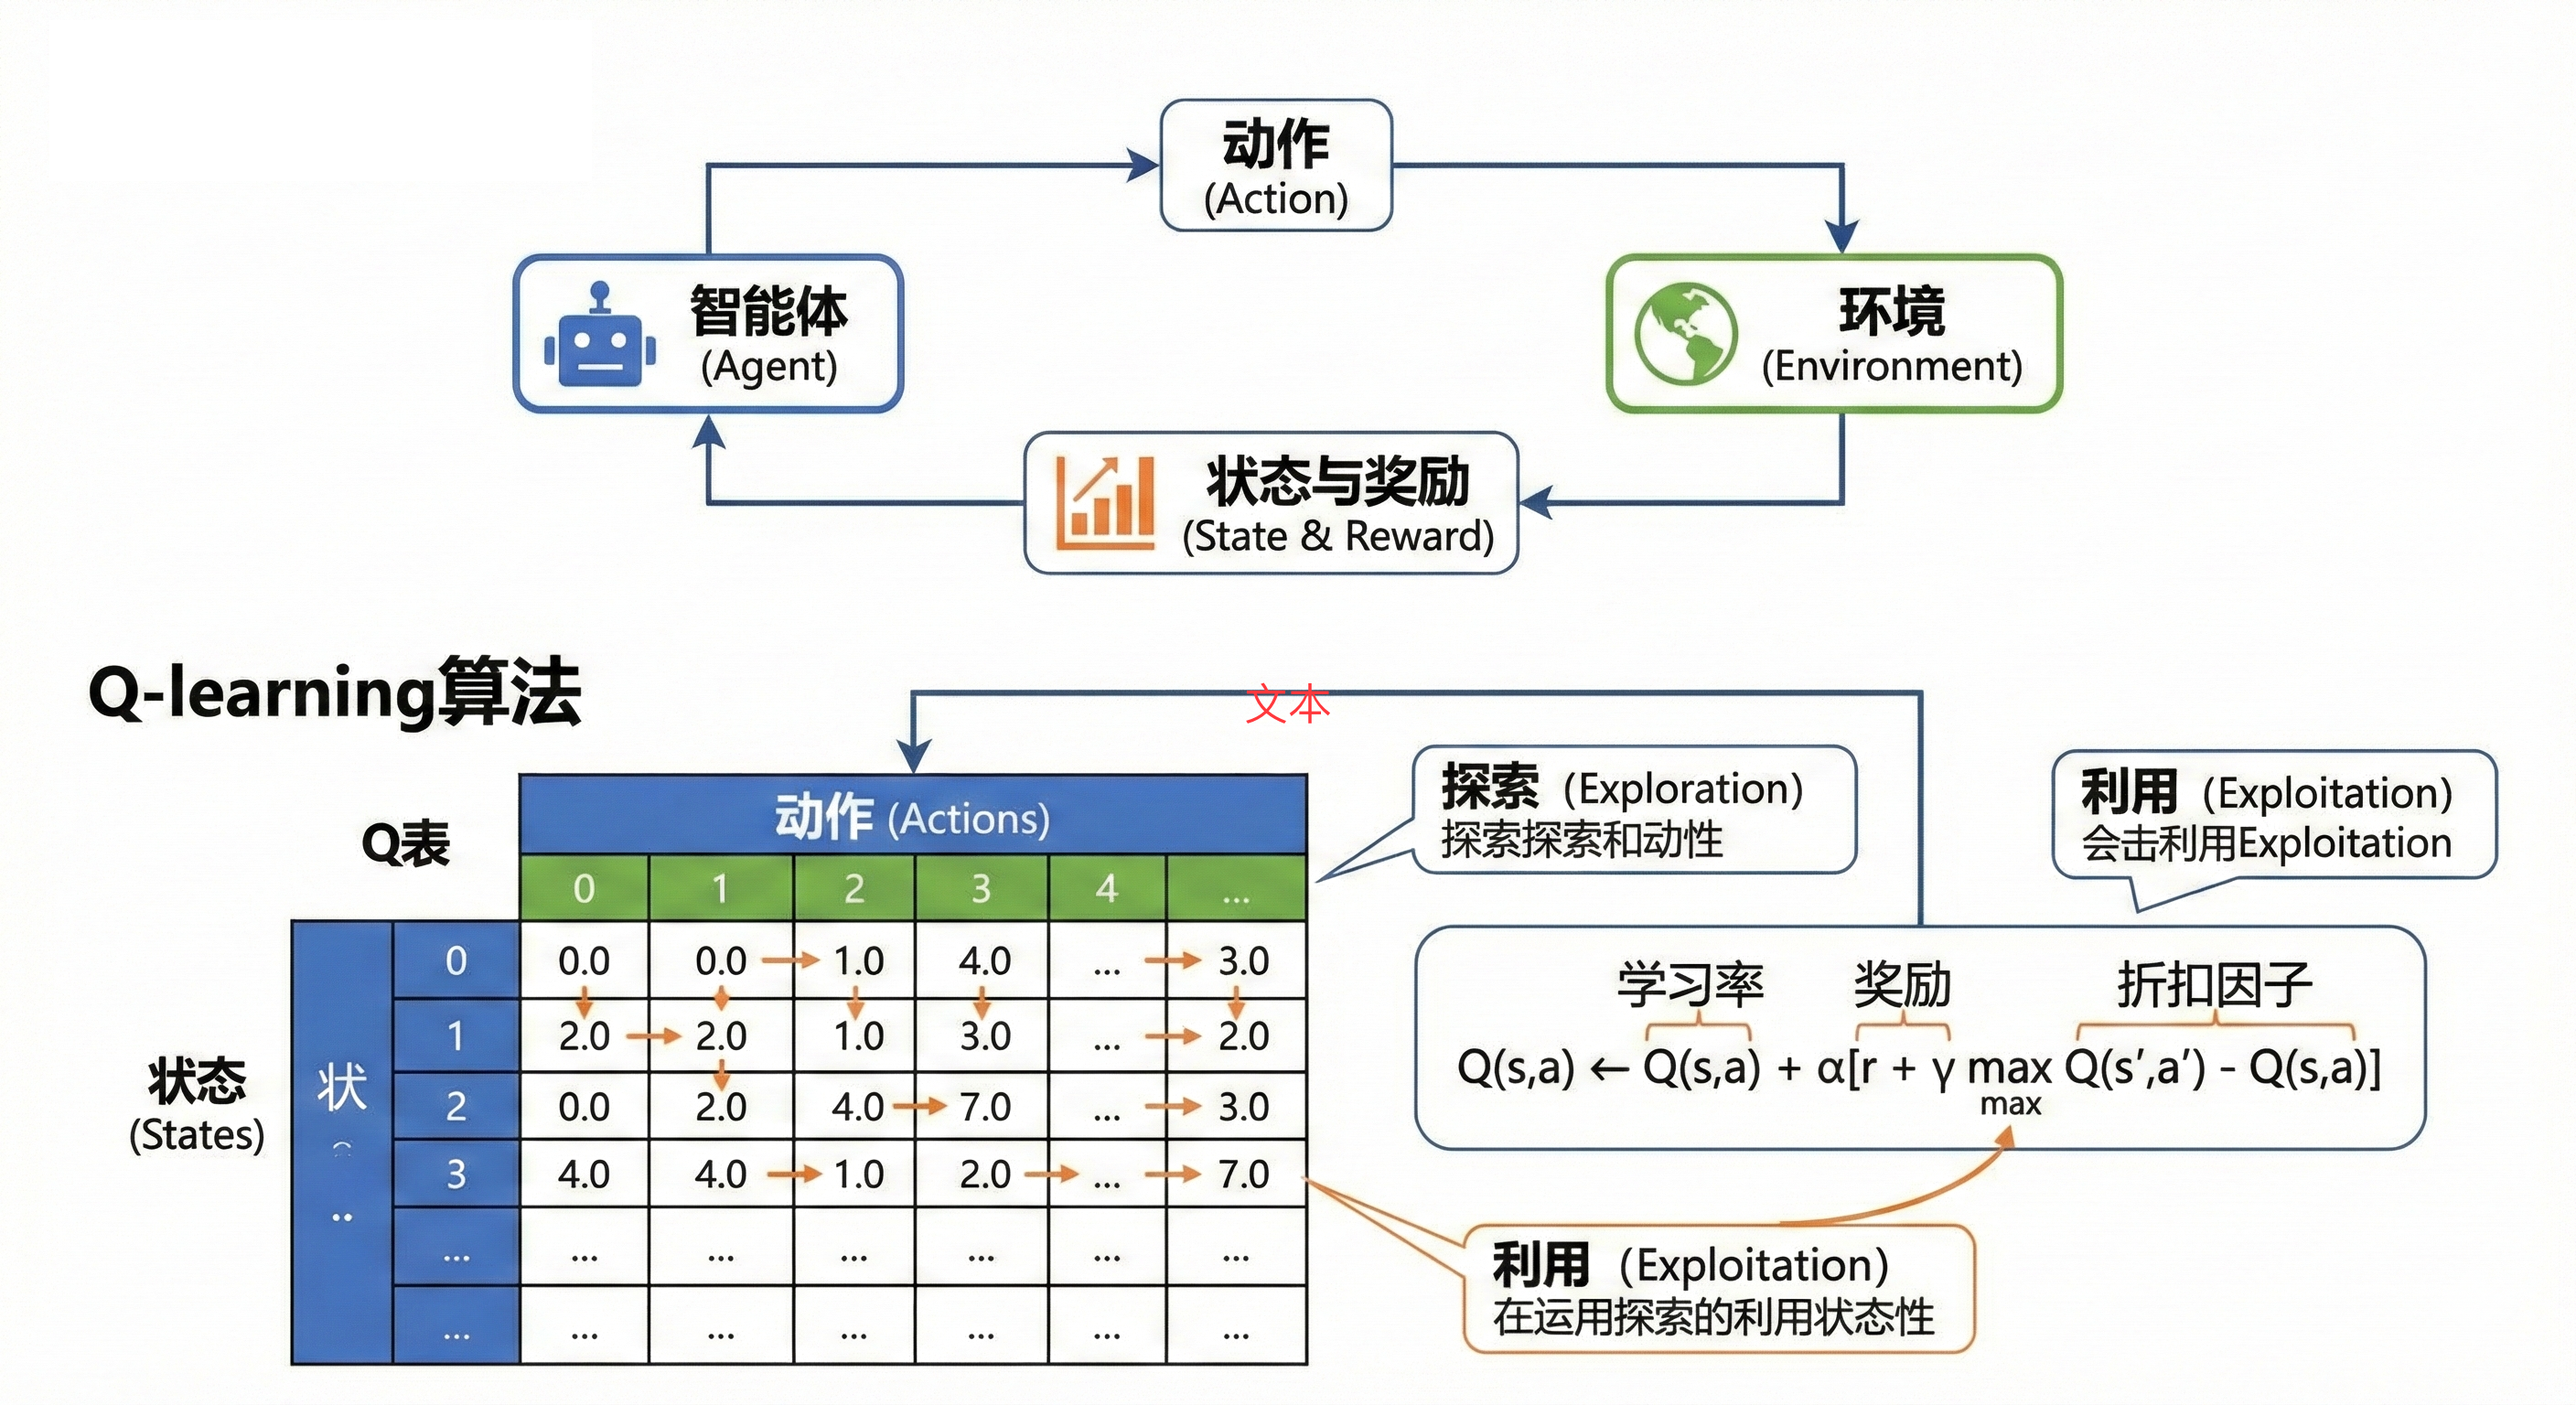
\includegraphics[width=0.75\textwidth]{figures/fig-3-3-4-reinforcement-learning.png}
\caption{\textbf{强化学习基本流程示意图}}
\label{fig:3-3-4-reinforcement-learning}
\end{figure}

\noindent \textbf{二\quad 一个经典的强化学习算法与计算实例}

\noindent 为了在不引入过多复杂背景的情况下展示强化学习的关键闭环,下面用最经典、最易于手算的算法之一:Q-learning,来讲解"策略如何改进"和"价值如何学习"。

\noindent \textbf{1)价值函数与最优性}

\noindent 强化学习里,一个核心概念是动作价值函数:
$Q^\pi(s,a)=\mathbb{E}_\pi\left[G_t\mid s_t=s,a_t=a\right],$
它表示在状态 $s$ 采取动作 $a$,并在之后遵循策略 $\pi$ 时能够获得的期望折扣回报。直观上,$Q$ 把"某个情境下做某个动作到底值不值"变成一个可比较的数。

\noindent 最优动作价值函数定义为
$Q^\ast(s,a)=\max_\pi Q^\pi(s,a),$
一旦知道 $Q^\ast$,最优策略就可以直接由"选 $Q$ 最大的动作"得到:
$\pi^\ast(s)=\arg\max_a Q^\ast(s,a).$

\noindent \textbf{2)Q-learning 的更新公式}

\noindent Q-learning 是一种离策略的时序差分方法。它不需要环境模型,也不需要给出正确动作标签,只要交互产生转移样本 $(s_t,a_t,r_{t+1},s_{t+1})$,就可以更新 $Q$:
$Q(s_t,a_t)\leftarrow Q(s_t,a_t)+\alpha\Big[r_{t+1}+\gamma\max_{a'}Q(s_{t+1},a')-Q(s_t,a_t)\Big],$
其中 $\alpha\in(0,1]$ 是学习率。

\noindent 这个式子的结构非常重要:它把"当前估计"与"更一致的估计"拉近。括号里的量
$\delta_t=r_{t+1}+\gamma\max_{a'}Q(s_{t+1},a')-Q(s_t,a_t)$
称为时序差分误差。它衡量的是:当前对 $Q(s_t,a_t)$ 的估计,与基于"一步奖励 $+$ 下一状态的最好价值"得到的估计之间差了多少。更新就是用 $\alpha$ 的比例去修正这个差距。

\noindent \textbf{3)一个可以手算的计算实例}

\noindent 考虑一个极简环境,只有两个非终止状态 $A,B$,以及一个终止状态 $T$。在状态 $A$ 有两个动作:$L$ 和 $R$。

\noindent 设定环境规则如下:
\begin{itemize}
\itemsep0pt
\item 在 $A$ 执行动作 $L$:转移到 $B$,获得奖励 $r=0$;
\item 在 $A$ 执行动作 $R$:直接到终止状态 $T$,获得奖励 $r=1$;
\item 在 $B$ 只有一个动作(可记为 $U$):到终止状态 $T$,获得奖励 $r=2$。
\end{itemize}

\noindent 取折扣因子 $\gamma=0.9$,学习率 $\alpha=1$(为了手算清晰,相当于每次直接用新估计覆盖旧值),并初始化所有 $Q$ 为 $0$:
$Q(A,L)=0,\quad Q(A,R)=0,\quad Q(B,U)=0.$

\noindent 现在假设智能体经历两条交互样本(这两条样本可以来自探索策略):

\noindent 第一条:在 $A$ 选择 $L$,到达 $B$,奖励 $0$。即 $(s=A,a=L,r=0,s'=B)$。更新:
$Q(A,L)\leftarrow 0 + \Big[0+0.9\max_{a'}Q(B,a')-0\Big]$
$=0.9\,Q(B,U)=0.$
因为此时 $Q(B,U)=0$,所以 $Q(A,L)$ 仍为 $0$。此时模型还不知道从 $B$ 能拿到好处。

\noindent 第二条:在 $B$ 执行动作 $U$,到达终止,奖励 $2$。即 $(s=B,a=U,r=2,s'=T)$。终止状态后续价值记为 $0$,因此
$Q(B,U)\leftarrow 0 + [2+0.9\cdot 0-0]=2.$
这一步把"在 $B$ 做 $U$ 值 $2$"学到了。

\noindent 如果此后再次经历一次从 $A$ 做 $L$ 到 $B$ 的样本(同样 $(A,L,0,B)$),更新会变为
$Q(A,L)\leftarrow 0 + [0+0.9\max_{a'}Q(B,a')-0]$
$=0.9\times 2=1.8.$
此时模型明白:虽然在 $A$ 做 $L$ 立刻没有奖励,但它把你带到 $B$,而在 $B$ 可以拿到 $2$ 的奖励,所以从长期看 $A$ 的 $L$ 是很有价值的。

\noindent 再对比 $A$ 的动作 $R$。若经历样本 $(A,R,1,T)$,则
$Q(A,R)\leftarrow 0+[1+0.9\cdot 0-0]=1.$
于是学到的价值为 $Q(A,L)=1.8$ 大于 $Q(A,R)=1$,因此在状态 $A$ 下更应选择 $L$ 而不是 $R$。这个例子恰好体现了强化学习的核心:好的行为不一定带来即时奖励,它可能通过未来的路径产生更大的长期回报;Q-learning 正是用"当前奖励 $+$ 下一步最优价值"的方式把延迟收益逐步向前传播。

\noindent \textbf{4)代码实现}

\noindent 下面用Python代码实现Q-learning的核心更新过程。这段代码与手算实例完全对应,环境包含状态 $A,B$ 和终止状态 $T$,动作有 $L,R,U$。

\begin{lstlisting}[language=Python, caption={Q-learning更新的Python实现}]
import numpy as np

# 状态和动作
states = ['A', 'B', 'T']  # T是终止状态
actions_A = ['L', 'R']     # 状态A的动作
actions_B = ['U']          # 状态B的动作

# 初始化Q值表(所有状态-动作对的初始值都为0)
Q = {
    'A': {'L': 0.0, 'R': 0.0},
    'B': {'U': 0.0},
    'T': {}
}

# 参数设置
gamma = 0.9   # 折扣因子
alpha = 1.0   # 学习率

# 定义环境转移函数:返回(下一状态, 奖励)
def step(state, action):
    if state == 'A' and action == 'L':
        return 'B', 0    # A->L转移到B,奖励0
    elif state == 'A' and action == 'R':
        return 'T', 1    # A->R直接到T,奖励1
    elif state == 'B' and action == 'U':
        return 'T', 2    # B->U到T,奖励2
    return 'T', 0

# Q-learning更新函数
def q_update(state, action, reward, next_state):
    # 获取下一状态的最大Q值
    if next_state == 'T' or len(Q[next_state]) == 0:
        max_q_next = 0  # 终止状态的价值为0
    else:
        max_q_next = max(Q[next_state].values())

    # 计算时序差分误差
    td_error = reward + gamma * max_q_next - Q[state][action]

    # 更新Q值
    Q[state][action] += alpha * td_error

# 经历第一条样本:(A, L, 0, B)
print("=== 第一条样本 (A, L, 0, B) ===")
next_state, reward = step('A', 'L')
q_update('A', 'L', reward, next_state)
print(f"Q(A,L) = {Q['A']['L']}")  # 输出: 0.0

# 经历第二条样本:(B, U, 2, T)
print("\n=== 第二条样本 (B, U, 2, T) ===")
next_state, reward = step('B', 'U')
q_update('B', 'U', reward, next_state)
print(f"Q(B,U) = {Q['B']['U']}")  # 输出: 2.0

# 再次经历样本:(A, L, 0, B)
print("\n=== 再次经历样本 (A, L, 0, B) ===")
next_state, reward = step('A', 'L')
q_update('A', 'L', reward, next_state)
print(f"Q(A,L) = {Q['A']['L']}")  # 输出: 1.8

# 经历样本:(A, R, 1, T)
print("\n=== 样本 (A, R, 1, T) ===")
next_state, reward = step('A', 'R')
q_update('A', 'R', reward, next_state)
print(f"Q(A,R) = {Q['A']['R']}")  # 输出: 1.0

# 比较两个动作的价值
print("\n=== 最终Q值 ===")
print(f"Q(A,L) = {Q['A']['L']}")
print(f"Q(A,R) = {Q['A']['R']}")
print(f"最优动作: {'L' if Q['A']['L'] > Q['A']['R'] else 'R'}")
\end{lstlisting}

\noindent \textbf{三\quad 强化学习中的关键难点与实践要点}

\noindent 强化学习在形式上很优美,但实践中比监督学习更脆弱,原因主要来自交互与延迟信号。

\noindent 探索与利用的权衡是不可回避的。如果总是选择当前 $Q$ 最大的动作(纯利用),就可能错过更优策略;如果探索太多,又会浪费样本并降低短期表现。常见的处理是 $\varepsilon$-greedy:以概率 $\varepsilon$ 随机选动作探索,以 $1-\varepsilon$ 选择当前最优动作利用。

\noindent 奖励设计决定了学习方向。奖励过于稀疏会导致学习效率极低,奖励设计不当则会诱发"钻空子"的策略,使得智能体最大化的是奖励函数而非真实目标。在实际任务中,奖励塑形、约束、以及对安全性的额外惩罚项往往与算法同等重要。

\noindent 样本效率与稳定性是工程瓶颈。强化学习需要大量交互数据,真实环境下成本高且风险大,因此仿真与离线数据常被引入,但这又带来分布偏移和估计偏差问题。深度强化学习进一步引入函数逼近,虽然表达能力更强,但也可能带来更复杂的训练不稳定性。

\noindent 总结而言,强化学习学习的是一套"长期最优的行为规则",其数学对象通常围绕回报、价值函数与策略展开;其训练机制通常依赖交互经验、时序差分误差与探索策略。理解 Q-learning 的更新闭环,可以为理解更复杂的 Actor–Critic、策略梯度以及基于模型的规划方法奠定基础。
